% InverseNet: Benchmarking Operator Mismatch and Calibration
% Across Compressive Imaging Modalities
%
% LaTeX source - ECCV-style conference paper

\documentclass[runningheads]{llncs}
\usepackage[T1]{fontenc}
\usepackage{graphicx}
\usepackage{amsmath,amssymb}
\usepackage{booktabs}
\usepackage{multirow}
\usepackage{xcolor}
\usepackage{hyperref}
\usepackage{cleveref}
\usepackage{subcaption}
\usepackage{array}

% Custom column type for tables
\newcolumntype{C}[1]{>{\centering\arraybackslash}p{#1}}

% Color definitions for highlighting
\definecolor{bestcolor}{rgb}{0.0, 0.5, 0.0}
\definecolor{worstcolor}{rgb}{0.7, 0.0, 0.0}

\newcommand{\best}[1]{\textbf{#1}}
\newcommand{\worst}[1]{\textcolor{worstcolor}{#1}}

\begin{document}

\title{InverseNet: Benchmarking Operator Mismatch and Calibration Across Compressive Imaging Modalities}
\titlerunning{InverseNet: Operator Mismatch Benchmark}

\author{Chengshuai Yang\inst{1}\thanks{Correspondence: \texttt{integrityyang@gmail.com}} \and Xin Yuan\inst{1,2}\thanks{\texttt{xyuan@westlake.edu.cn}}}
\authorrunning{Yang \and Yuan}
\institute{NextGen PlatformAI C Corp, USA \and
School of Engineering, Westlake University, Hangzhou, China}

\maketitle

% ============================================================================
% ABSTRACT
% ============================================================================
\begin{abstract}
State-of-the-art EfficientSCI loses 20.58\,dB when its assumed forward operator deviates from physical reality by just eight parameters---yet no existing benchmark quantifies this \emph{operator mismatch}, which is the default condition of every deployed compressive imaging system.
We introduce \textbf{InverseNet}, the first cross-modality benchmark for operator mismatch, spanning CASSI, CACTI, and single-pixel cameras.
Evaluating 12 methods under a four-scenario protocol (ideal, mismatched, oracle-corrected, blind calibration) across 27 simulated scenes and 9 real hardware captures, we find: (1)~deep learning methods lose 10--21\,dB under mismatch, collapsing their advantage over classical baselines; (2)~an inverse performance--robustness relationship holds across modalities (Spearman $r_s{=}{-}0.71$, $p{<}0.01$); (3)~\emph{mask-oblivious} architectures recover 0\% of mismatch losses regardless of calibration quality, while \emph{operator-conditioned} methods recover 41--90\%; (4)~blind grid-search calibration recovers 85--100\% of the oracle bound without ground truth.
Real hardware experiments confirm simulation patterns transfer to physical data.
Code is available upon acceptance.

\keywords{Compressive imaging \and Operator mismatch \and Calibration \and Benchmark \and Spectral imaging \and Video compressive sensing \and Single-pixel camera}
\end{abstract}

% ============================================================================
% 1. INTRODUCTION
% ============================================================================
\section{Introduction}
\label{sec:intro}

Compressive imaging acquires fewer measurements than the Nyquist limit by exploiting signal structure, recovering the full signal through computational reconstruction.
This paradigm underlies diverse modalities including hyperspectral imaging via coded apertures~\cite{wagadarikar2008cassi,meng2020e2e}, video compressive sensing via temporal coding~\cite{llull2013cacti,yuan2021snapshot}, and single-pixel cameras via structured illumination~\cite{duarte2008spc,edgar2019spc_review}.
In all cases, reconstruction quality depends critically on knowledge of the forward measurement operator---the mapping from scene to measurements.

Yet a dangerous chasm separates research from reality.
Reconstruction algorithms are benchmarked with idealized forward operators, but deployed systems suffer \emph{operator mismatch}: EfficientSCI~\cite{wang2023efficientsci} collapses from 35.39 to 14.81\,dB---a 20.58\,dB drop---under realistic 8-parameter mismatch.
For CASSI, mask misalignment of 0.5\,px combined with 1\% dispersion drift degrades PSNR by over 13\,dB (\cref{tab:cassi}); for CACTI, spatial, temporal, and radiometric errors compound across 8~parameters; for single-pixel cameras, gain drift causes systematic errors.
These mismatches are ubiquitous yet systematically ignored in benchmarks.

\textbf{The benchmark gap.}
Just as CASP~\cite{moult2005casp} transformed protein folding by forcing blind prediction against nature, computational imaging needs benchmarks that evaluate against physical reality.
Existing benchmarks---KAIST~\cite{choi2017kaist} for CASSI, the CACTI benchmark~\cite{yuan2021snapshot}---assume perfect operator knowledge, providing no information about mismatch robustness.
Antun et al.~\cite{antun2020instabilities} showed deep learning solvers are unstable to adversarial perturbations; InverseNet operationalizes this for \emph{physically realistic} operator mismatch.

\textbf{Contributions.}
We address this gap with InverseNet, which makes four contributions:
\begin{enumerate}
    \item \textbf{Unified four-scenario protocol.} We define four scenarios---ideal~(I), mismatched~(II), oracle-corrected~(III), and blind calibration~(IV)---applicable across modalities. The I$\to$II gap quantifies mismatch sensitivity; II$\to$III quantifies calibration potential; IV measures practical recovery via self-supervised calibration.

    \item \textbf{Cross-modality benchmark.} We evaluate 12 methods (4 CASSI, 4 CACTI, 4 SPC) spanning classical, plug-and-play, and deep learning approaches across 27 simulated scenes, producing over 360 experiments.

    \item \textbf{Real hardware validation.} We validate simulation findings on 5 real CASSI scenes and 4 real CACTI scenes from publicly available hardware captures, confirming that mismatch patterns transfer to physical data.

    \item \textbf{Open dataset.} All reconstruction arrays, per-scene metrics, and analysis code will be publicly released.\footnote{Code available upon acceptance.} All test data come from existing public datasets.
\end{enumerate}

Our key findings include: (a)~operator mismatch degrades deep learning methods by 10--21\,dB while classical methods lose only 3--11\,dB; (b)~operator-aware architectures are simultaneously the most sensitive to mismatch and the most recoverable through calibration; (c)~mask-oblivious architectures show zero calibration benefit; (d)~CACTI exhibits the most severe degradation (up to 20.58\,dB) due to its 8-parameter mismatch space; (e)~dispersion mismatch in CASSI limits oracle recoverability due to fixed-step architectural assumptions.

% ============================================================================
% 2. RELATED WORK
% ============================================================================
\section{Related Work}
\label{sec:related}

\paragraph{Compressive imaging reconstruction.}
Classical methods employ convex optimization with sparsity priors: GAP-TV~\cite{yuan2016gaptv} for CASSI and CACTI, FISTA~\cite{beck2009fista} and ADMM~\cite{boyd2011admm} for general inverse problems.
Deep learning has dramatically improved quality: MST~\cite{cai2022mst} introduces mask-guided spectral transformers; HDNet~\cite{hu2022hdnet} uses dual-domain processing; DAUHST~\cite{cai2022dauhst} and RDLUF-MixS$^2$~\cite{li2023rdluf} further advance CASSI reconstruction.
For CACTI, EfficientSCI~\cite{wang2023efficientsci}, ELP-Unfolding~\cite{yang2022elp}, and DiffSCI~\cite{meng2024diffsci} achieve state-of-the-art results.
ISTA-Net~\cite{zhang2018istanet} and HATNet~\cite{qu2024hatnet} address single-pixel imaging.
All are evaluated assuming perfect forward operators.

\paragraph{Calibration and operator mismatch.}
Operator mismatch has been studied per-modality but not systematically benchmarked.
Wagadarikar et al.~\cite{wagadarikar2008cassi} and Arguello et al.~\cite{arguello2013cassi_calib} address CASSI mask calibration; fastMRI~\cite{zbontar2018fastmri} evaluates MRI undersampling but assumes known coil sensitivities.
Learned reconstruction~\cite{adler2018learned} and plug-and-play methods~\cite{ryu2019pnp} focus on signal priors rather than operator fidelity.
Berk et al.~\cite{berk2024robust} provide theoretical error bounds under structured model mismatch, consistent with our empirical observations.
No prior work offers a unified cross-modality benchmark quantifying both mismatch degradation and calibration recovery.

\paragraph{Reconstruction benchmarks.}
The KAIST TSA dataset~\cite{choi2017kaist} (CASSI), the CACTI benchmark~\cite{yuan2021snapshot}, and Set11~\cite{kulkarni2016reconnet} (SPC) are standard evaluation suites.
Large-scale benchmarks like NTIRE~\cite{timofte2017ntire} and SupER~\cite{kohler2020super} standardize restoration evaluation but do not enable controlled forward-model modification.
InverseNet extends these by introducing controlled operator mismatch and measuring calibration recovery.

% ============================================================================
% 3. THE INVERSENET BENCHMARK
% ============================================================================
\section{The InverseNet Benchmark}
\label{sec:benchmark}

\subsection{Unified Four-Scenario Protocol}
\label{sec:protocol}

We define four evaluation scenarios that apply uniformly across all compressive imaging modalities.
Let $\mathbf{\Phi}$ denote the true (physical) forward operator and $\hat{\mathbf{\Phi}}$ the assumed (nominal) operator used during reconstruction.

\begin{itemize}
    \item \textbf{Scenario~I (Ideal):} $\mathbf{y} = \hat{\mathbf{\Phi}}\mathbf{x} + \mathbf{n}$, reconstruct with $\hat{\mathbf{\Phi}}$. Best-case performance with perfect operator knowledge.

    \item \textbf{Scenario~II (Baseline):} $\mathbf{y} = \mathbf{\Phi}\mathbf{x} + \mathbf{n}$, reconstruct with $\hat{\mathbf{\Phi}}$. Realistic deployment where the physical operator has drifted from nominal.

    \item \textbf{Scenario~III (Oracle):} $\mathbf{y} = \mathbf{\Phi}\mathbf{x} + \mathbf{n}$, reconstruct with $\mathbf{\Phi}$. Upper bound achievable through perfect calibration.

    \item \textbf{Scenario~IV (Blind Calibration):} $\mathbf{y} = \mathbf{\Phi}\mathbf{x} + \mathbf{n}$, reconstruct with $\tilde{\mathbf{\Phi}}$ estimated via grid search over mismatch parameters using a self-supervised objective (measurement residual for geometric mismatch, reconstruction sparsity for radiometric mismatch). Practical calibration without ground truth.
\end{itemize}

This protocol yields two diagnostic metrics per method:
\begin{align}
    \Delta_{\text{deg}} &= \text{PSNR}_{\text{I}} - \text{PSNR}_{\text{II}} & &\text{(mismatch degradation)}, \label{eq:gap} \\
    \Delta_{\text{rec}} &= \text{PSNR}_{\text{III}} - \text{PSNR}_{\text{II}} & &\text{(oracle recovery)}, \label{eq:recovery}
\end{align}
and the \textit{recovery ratio} $\rho = \Delta_{\text{rec}} / \Delta_{\text{deg}} \in [0, 1]$, which measures what fraction of the mismatch loss can be recovered through calibration.

\subsection{CASSI: Coded Aperture Snapshot Spectral Imaging}
\label{sec:cassi}

\paragraph{Forward model.}
CASSI acquires a 2D measurement $\mathbf{y} \in \mathbb{R}^{H \times W'}$ of a 3D hyperspectral cube $\mathbf{x} \in \mathbb{R}^{H \times W \times \Lambda}$ through a coded aperture mask $\mathbf{M} \in \{0,1\}^{H \times W}$ followed by a dispersive prism.
The measurement at pixel $(i, j)$ is:
\begin{equation}
    y(i, j) = \sum_{\lambda=1}^{\Lambda} M(i, j - d(\lambda)) \cdot x(i, j, \lambda) + n(i, j),
    \label{eq:cassi_forward}
\end{equation}
where $d(\lambda)$ is the dispersion shift for spectral band $\lambda$ and $W' = W + (\Lambda - 1) \cdot s$ with dispersion step $s$.

\paragraph{Mismatch model.}
We model CASSI operator mismatch as a 5-parameter perturbation combining mask misalignment and dispersion drift:
\begin{equation}
    \mathbf{\Phi} = \mathcal{D}(a_1, \alpha) \circ \mathcal{T}(dx, dy, \theta) \circ \hat{\mathbf{\Phi}},
\end{equation}
where $dx, dy$ are subpixel translational shifts, $\theta$ is a rotational misalignment of the coded aperture mask, $a_1$ is the dispersion slope (nominal $s = 2.0$\,px/band), and $\alpha$ is the dispersion axis angular offset.
We use $dx = 0.5$\,px, $dy = 0.3$\,px, $\theta = 0.1^\circ$ for mask misalignment, and $a_1 = 2.02$\,px/band (1\% drift from nominal) and $\alpha = 0.15^\circ$ for dispersion mismatch, representing moderate assembly and optical tolerances.

\paragraph{Reconstruction methods.}
We evaluate four methods:
\textbf{GAP-TV}~\cite{yuan2016gaptv}: classical accelerated proximal gradient with TV regularization (100 iterations, $\lambda_{\text{TV}} = 0.1$);
\textbf{PnP-HSICNN}~\cite{zheng2021pnp}: plug-and-play GAP with HSI-SDeCNN deep denoiser (124 iterations: TV iters 0--82, HSICNN iters 83--123);
\textbf{HDNet}~\cite{hu2022hdnet}: dual-domain deep network with spectral discrimination learning (pretrained);
\textbf{MST-L}~\cite{cai2022mst}: mask-guided spectral transformer, large variant (2 stages, blocks $[4,7,5]$, pretrained).

\paragraph{Dataset.}
We use 10 scenes from the KAIST TSA simulated dataset~\cite{choi2017kaist}, each consisting of a $256 \times 256 \times 28$ hyperspectral cube spanning 450--650\,nm.
Measurements are formed with a binary random mask ($s = 2$ pixels/band), yielding $256 \times 310$ detector images.
Low noise ($\alpha = 10^5$ photon peak, $\sigma = 0.01$ read noise) isolates the effect of operator mismatch.

\subsection{CACTI: Coded Aperture Compressive Temporal Imaging}
\label{sec:cacti}

\paragraph{Forward model.}
CACTI acquires a single 2D snapshot $\mathbf{y} \in \mathbb{R}^{H \times W}$ encoding $B$ high-speed video frames $\mathbf{x} \in \mathbb{R}^{H \times W \times B}$ through a dynamic coded aperture:
\begin{equation}
    y(i, j) = \sum_{b=1}^{B} C_b(i, j) \cdot x(i, j, b) + n(i, j),
    \label{eq:cacti_forward}
\end{equation}
where $C_b \in \{0,1\}^{H \times W}$ is the binary mask pattern for temporal frame $b$.

\paragraph{Mismatch model.}
CACTI mismatch involves 8 parameters capturing spatial, temporal, and radiometric errors:
spatial shifts ($dx = 0.5$\,px, $dy = 0.3$\,px), rotation ($\theta = 0.1^\circ$), temporal clock offset ($\Delta t = 0.05$), duty cycle deviation ($\eta = 0.95$), detector gain ($g = 1.02$), offset ($o = 0.002$), and measurement noise ($\sigma_n = 1.0$).

\paragraph{Reconstruction methods.}
We evaluate four methods:
\textbf{GAP-TV}~\cite{yuan2016gaptv}: classical iterative with TV regularization;
\textbf{PnP-FFDNet}~\cite{yuan2020pnp}: plug-and-play with FFDNet denoiser;
\textbf{ELP-Unfolding}~\cite{yang2022elp}: ensemble learning priors driven deep unfolding network (pretrained);
\textbf{EfficientSCI}~\cite{wang2023efficientsci}: efficient deep learning for snapshot compressive imaging (pretrained).

\paragraph{Dataset.}
We use 6 standard benchmark videos (\textit{kobe}, \textit{traffic}, \textit{runner}, \textit{drop}, \textit{crash}, \textit{aerial}) at $256 \times 256$ resolution with $B = 8$ temporal frames per snapshot, following the standard video compressive sensing evaluation protocol~\cite{yuan2021snapshot}.

\subsection{SPC: Single-Pixel Camera}
\label{sec:spc}

\paragraph{Forward model.}
The single-pixel camera acquires $m$ scalar measurements of an image $\mathbf{x} \in \mathbb{R}^{n}$ through structured illumination patterns:
\begin{equation}
    \mathbf{y} = \mathbf{A}\mathbf{x} + \mathbf{n},
    \label{eq:spc_forward}
\end{equation}
where $\mathbf{A} \in \mathbb{R}^{m \times n}$ is the measurement matrix (typically Gaussian or Hadamard patterns) with compression ratio $m/n$.

\paragraph{Mismatch model.}
We model SPC mismatch as exponential gain drift affecting the measurement rows:
\begin{equation}
    \mathbf{\Phi} = \text{diag}\!\left(e^{-\alpha \cdot \mathbf{i}}\right) \cdot \hat{\mathbf{\Phi}},
\end{equation}
where $\alpha = 0.0015$ controls the drift rate and $\mathbf{i} = [0, 1, \ldots, m{-}1]^{\!\top}$ indexes the measurement rows, modelling progressive detector gain decay during sequential acquisition.
Additional measurement noise $\sigma_y = 0.03$ is applied.

\paragraph{Reconstruction methods.}
We evaluate four methods:
\textbf{FISTA-TV}~\cite{beck2009fista}: fast iterative shrinkage-thresholding with TV regularization (500 iterations, $\lambda = 0.005$);
\textbf{PnP-DRUNet}~\cite{zhang2021drunet}: plug-and-play FISTA with DRUNet denoiser and sigma annealing (200 iterations, row-normalized operator);
\textbf{ISTA-Net}~\cite{zhang2018istanet}: learned iterative shrinkage-thresholding network (pretrained);
\textbf{HATNet}~\cite{qu2024hatnet}: dual-scale transformer for single-pixel imaging (pretrained).

\paragraph{Dataset.}
We use the 11 standard Set11 test images (\textit{Monarch}, \textit{Parrots}, \textit{barbara}, \textit{boats}, \textit{cameraman}, \textit{fingerprint}, \textit{flinstones}, \textit{foreman}, \textit{house}, \textit{lena256}, \textit{peppers256}) at $256 \times 256$ resolution with 25\% sampling ratio.

\subsection{Evaluation Metrics}
\label{sec:metrics}

We report three standard image quality metrics:
\begin{itemize}
    \item \textbf{PSNR} (peak signal-to-noise ratio, dB): pixel-level fidelity, computed per-channel and averaged.
    \item \textbf{SSIM} (structural similarity index): perceptual structural quality~\cite{wang2004ssim}.
    \item \textbf{SAM} (spectral angle mapper, degrees): spectral fidelity, reported for CASSI only.
\end{itemize}

% ============================================================================
% 4. EXPERIMENTAL RESULTS
% ============================================================================
\section{Experimental Results}
\label{sec:results}

\begin{figure}[t]
\centering
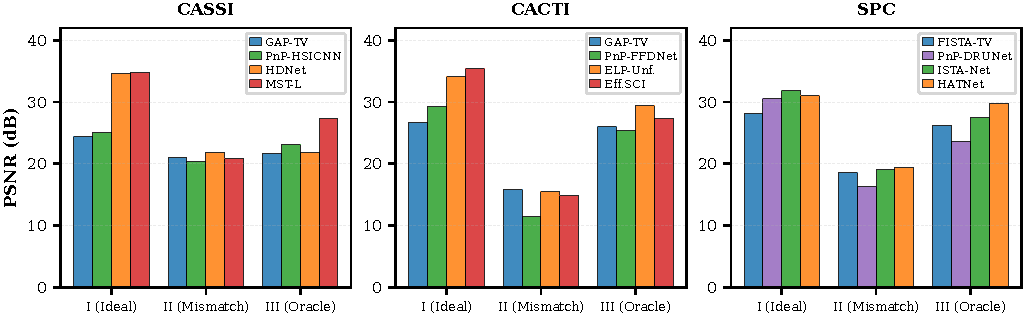
\includegraphics[width=\textwidth]{figures/fig1_scenario_comparison.pdf}
\caption{PSNR across three scenarios for all modalities. Scenario~I (Ideal): perfect operator. Scenario~II (Baseline): mismatched operator. Scenario~III (Oracle): true operator used for reconstruction. The collapse of deep learning methods under Scenario~II is visible across all modalities, with CACTI showing the most severe degradation.}
\label{fig:scenario_comparison}
\end{figure}

\begin{figure}[t]
\centering
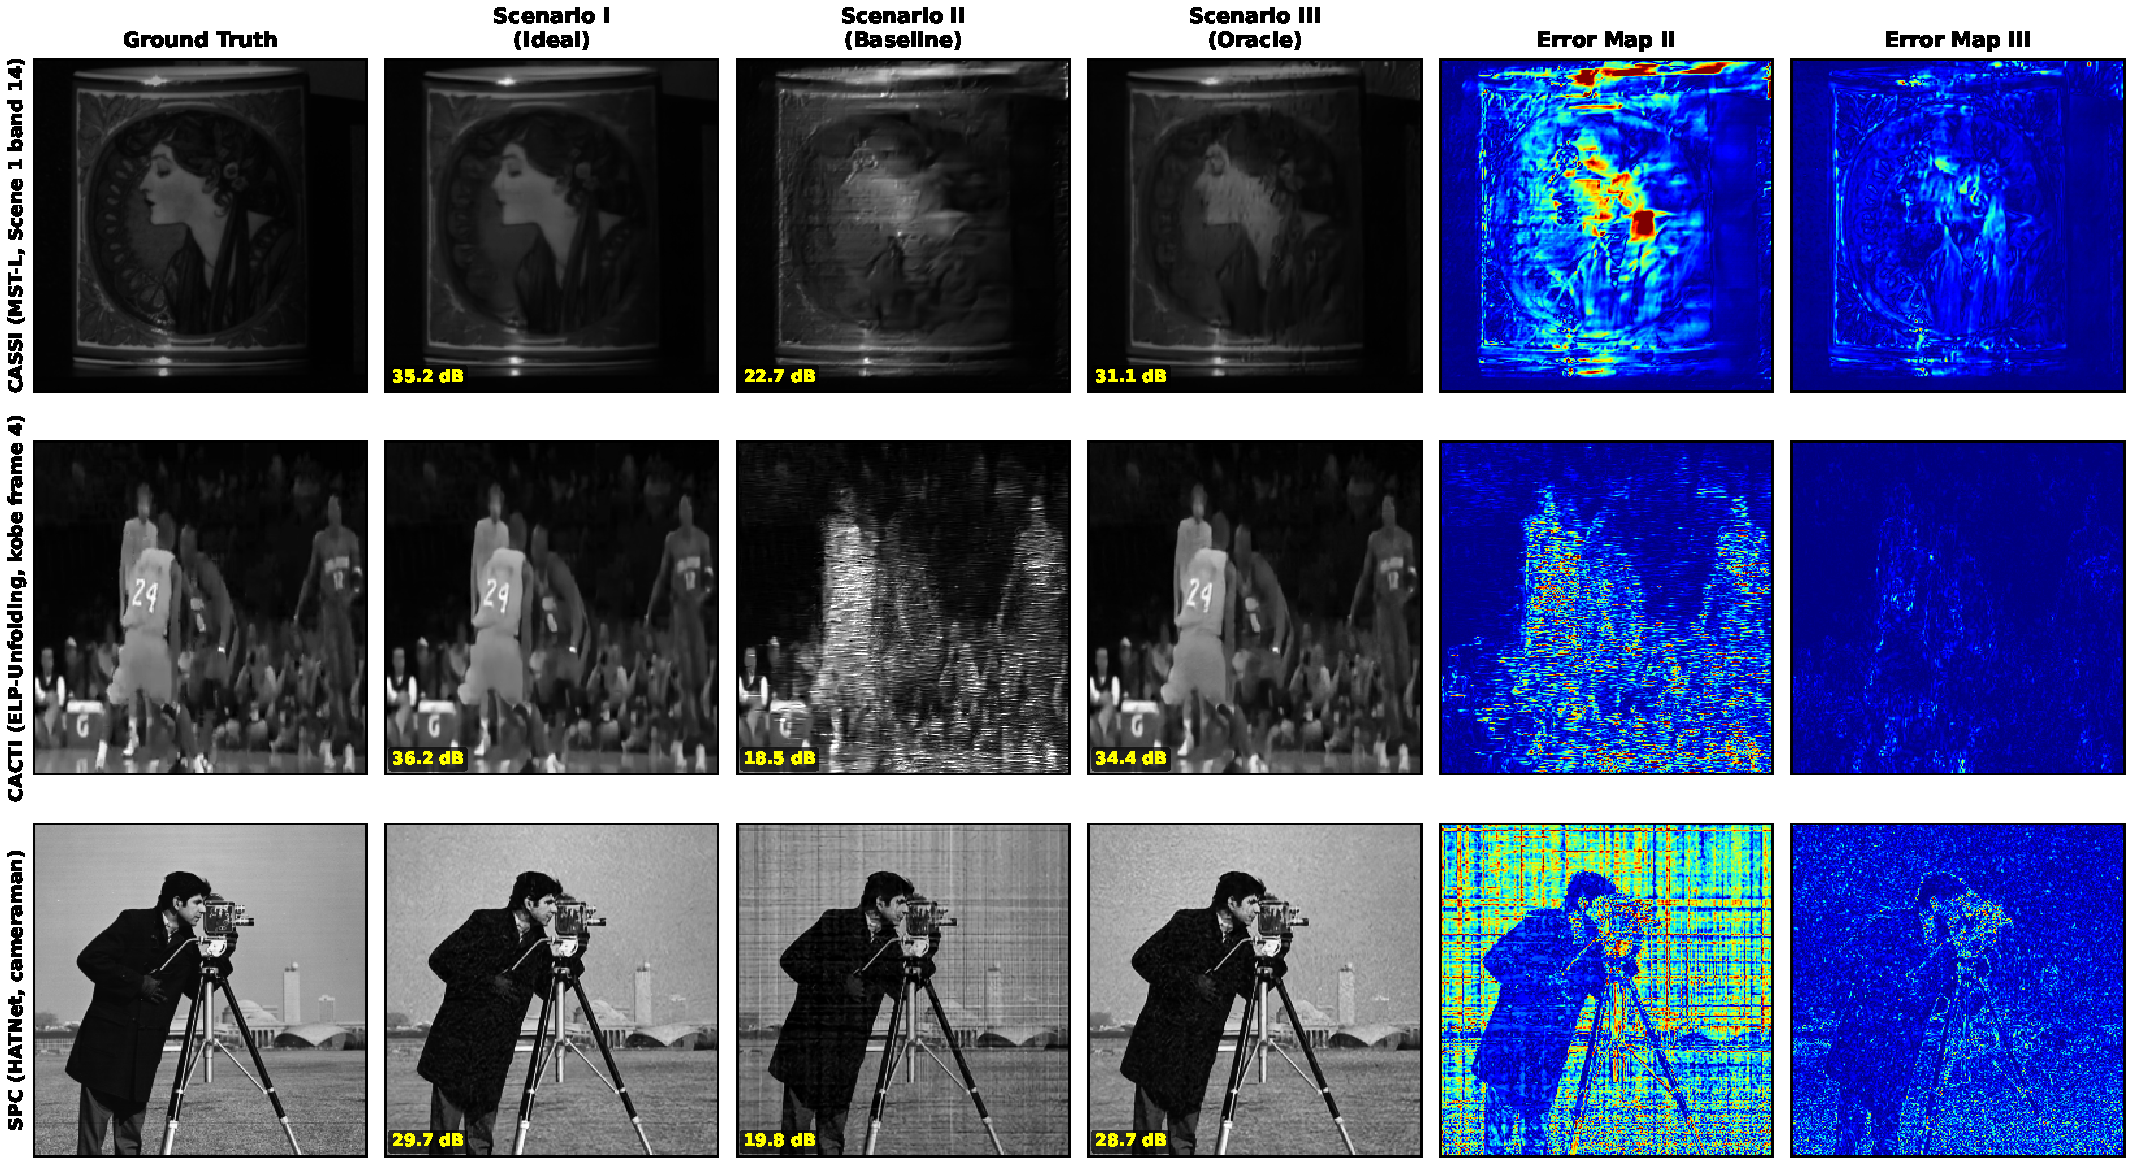
\includegraphics[width=\textwidth]{figures/visual_comparison.pdf}
\caption{Qualitative reconstruction comparison across three modalities. Each row shows a representative scene for one modality (CASSI: Scene~1 band~14, MST-L; CACTI: \textit{kobe} frame~4, ELP-Unfolding; SPC: \textit{cameraman}, HATNet). Error maps (jet colormap, same scale per row) highlight how mismatch (Scenario~II) introduces spatially structured artifacts that oracle correction (Scenario~III) largely removes.}
\label{fig:visual_comparison}
\end{figure}

\subsection{CASSI Results}
\label{sec:cassi_results}

\Cref{fig:visual_comparison} provides qualitative examples of reconstruction degradation and recovery across all three modalities.
\Cref{tab:cassi} presents the CASSI benchmark results across 10 KAIST scenes (\cref{fig:scenario_comparison}).

\begin{table}[t]
\centering
\caption{CASSI reconstruction results (10 KAIST scenes, $256 \times 256 \times 28$, 5-parameter mismatch). PSNR (dB) / SSIM reported as mean $\pm$ std. $\Delta_{\text{deg}}$: degradation (I$\rightarrow$II). $\Delta_{\text{rec}}$: oracle recovery (II$\rightarrow$III). $\rho$: recovery ratio. Best Scenario~I and~III PSNR in \textbf{bold}; best $\rho$ marked with $\dagger$.}
\label{tab:cassi}
\resizebox{\textwidth}{!}{%
\begin{tabular}{@{}lcccccc@{}}
\toprule
\textbf{Method} & \textbf{Scenario I} & \textbf{Scenario II} & \textbf{Scenario III} & $\boldsymbol{\Delta}_{\textbf{deg}}$ & $\boldsymbol{\Delta}_{\textbf{rec}}$ & $\boldsymbol{\rho}$ \\
\midrule
GAP-TV~\cite{yuan2016gaptv}
 & 24.34{\scriptsize$\pm$1.90} / .722
 & 20.96{\scriptsize$\pm$1.62} / .611
 & 21.72{\scriptsize$\pm$1.48} / .687
 & 3.38 & 0.76 & 22.5\% \\
PnP-HSICNN~\cite{zheng2021pnp}
 & 25.12{\scriptsize$\pm$1.88} / .758
 & 20.40{\scriptsize$\pm$1.71} / .574
 & 23.08{\scriptsize$\pm$1.52} / .702
 & 4.72 & 2.68 & \best{56.8\%}$^\dagger$ \\
HDNet~\cite{hu2022hdnet}
 & 34.66{\scriptsize$\pm$2.62} / .970
 & 21.88{\scriptsize$\pm$1.72} / .756
 & 21.88{\scriptsize$\pm$1.72} / .756
 & 12.78 & 0.00 & 0\% \\
MST-L~\cite{cai2022mst}
 & \textbf{34.81}{\scriptsize$\pm$2.11} / \textbf{.973}
 & 20.83{\scriptsize$\pm$2.01} / .744
 & \textbf{27.33}{\scriptsize$\pm$1.86} / \textbf{.881}
 & 13.98 & \best{6.50} & 46.5\% \\
\bottomrule
\end{tabular}%
}
\end{table}

\paragraph{Key findings.}
The CASSI results reveal a dichotomy between operator-aware and mask-oblivious architectures.
\textbf{PnP-HSICNN} achieves the highest oracle recovery ratio ($\rho = 56.8\%$, +2.68\,dB), outperforming even the deep \textbf{MST-L} ($\rho = 46.5\%$, +6.50\,dB absolute), because its iterative GAP backbone directly benefits from corrected mask and dispersion parameters.
\textbf{HDNet} shows \textit{zero} oracle gain ($\Delta_{\text{rec}} = 0.00$\,dB), confirming mask-oblivious architectures cannot benefit from calibration.
Under Scenario~II, all methods converge to 20.40--21.88\,dB, erasing the ${\sim}$10\,dB ideal-condition advantage of deep learning over classical methods.

\begin{figure}[t]
\centering
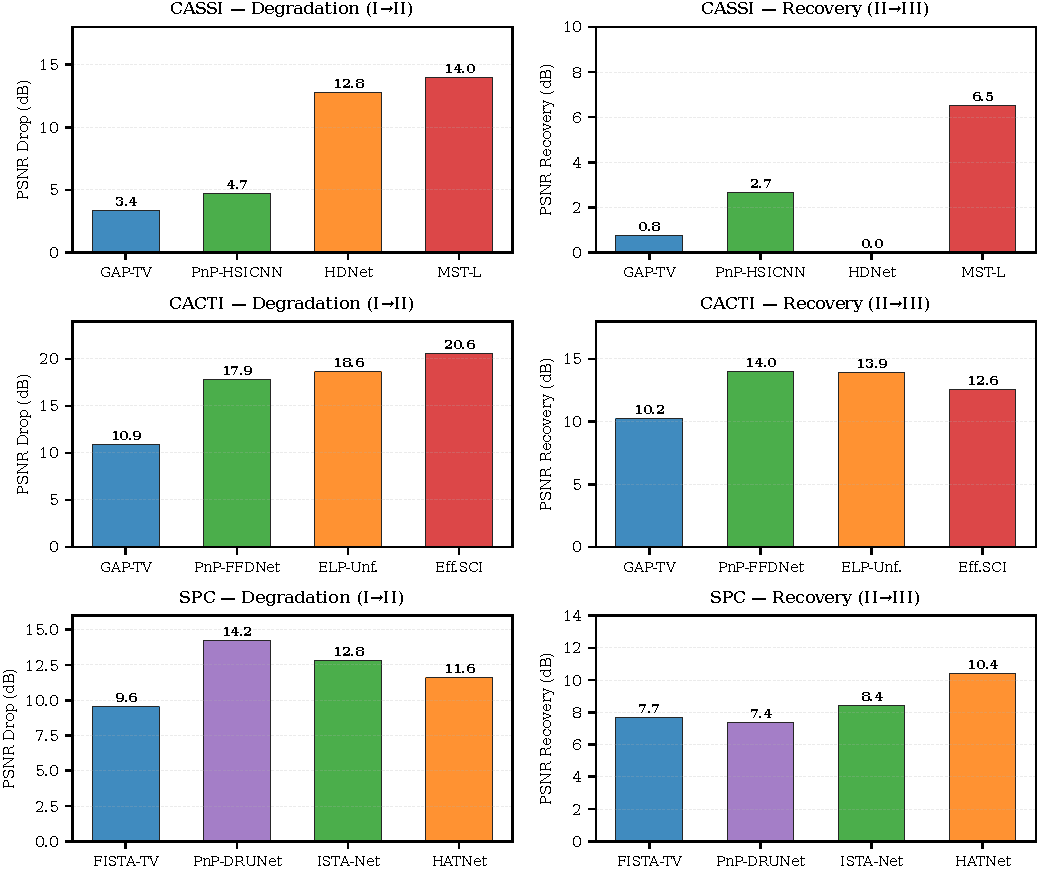
\includegraphics[width=\textwidth]{figures/fig3_gap_comparison.pdf}
\caption{Mismatch degradation ($\Delta_{\text{deg}}$, left) and oracle recovery ($\Delta_{\text{rec}}$, right) per method across all three modalities. CACTI suffers the most severe degradation (up to 20.6\,dB) but also the highest absolute recovery. For CASSI, HDNet shows zero recovery due to its mask-oblivious architecture; PnP-HSICNN achieves the best recovery ratio ($\rho = 56.8\%$). For SPC, HATNet recovers 10.4\,dB ($\rho = 89.6\%$).}
\label{fig:gap_comparison}
\end{figure}

\subsection{CACTI Results}
\label{sec:cacti_results}

\Cref{tab:cacti} presents the CACTI benchmark results across 6 standard benchmark videos (\cref{fig:scenario_comparison}).

\begin{table}[t]
\centering
\caption{CACTI reconstruction results (6 videos, $256 \times 256 \times 8$). PSNR (dB) / SSIM reported as mean $\pm$ std. CACTI exhibits the most severe mismatch degradation of all three modalities.}
\label{tab:cacti}
\resizebox{\textwidth}{!}{%
\begin{tabular}{@{}lcccccc@{}}
\toprule
\textbf{Method} & \textbf{Scenario I} & \textbf{Scenario II} & \textbf{Scenario III} & $\boldsymbol{\Delta}_{\textbf{deg}}$ & $\boldsymbol{\Delta}_{\textbf{rec}}$ & $\boldsymbol{\rho}$ \\
\midrule
GAP-TV~\cite{yuan2016gaptv}
 & 26.75{\scriptsize$\pm$4.48} / .848
 & 15.81{\scriptsize$\pm$1.98} / .305
 & 26.01{\scriptsize$\pm$3.72} / .794
 & 10.94 & \best{10.21} & \best{93.3\%} \\
PnP-FFDNet~\cite{yuan2020pnp}
 & 29.28{\scriptsize$\pm$5.53} / .890
 & 11.43{\scriptsize$\pm$2.71} / .216
 & 25.39{\scriptsize$\pm$3.52} / .820
 & 17.85 & 13.96 & 78.2\% \\
ELP-Unfolding~\cite{yang2022elp}
 & 34.09{\scriptsize$\pm$4.11} / .965
 & 15.47{\scriptsize$\pm$1.71} / .308
 & 29.40{\scriptsize$\pm$3.15} / .927
 & 18.63 & 13.93 & 74.8\% \\
EfficientSCI~\cite{wang2023efficientsci}
 & \textbf{35.39}{\scriptsize$\pm$4.46} / \textbf{.973}
 & 14.81{\scriptsize$\pm$2.19} / .303
 & 27.38{\scriptsize$\pm$3.52} / .927
 & 20.58 & 12.57 & 61.1\% \\
\bottomrule
\end{tabular}%
}
\end{table}

\paragraph{Key findings.}
CACTI exhibits the most severe mismatch degradation, with losses from 10.94\,dB (GAP-TV) to 20.58\,dB (EfficientSCI).
The 8-parameter mismatch space creates compounding degradation; under Scenario~II all methods collapse to 11--16\,dB (SSIM~$<$~0.31).
\textbf{GAP-TV} achieves the highest recovery ratio ($\rho = 93.3\%$), while \textbf{EfficientSCI} has the lowest (61.1\%) despite best ideal PSNR, suggesting learned features are partially coupled to the ideal operator.

\paragraph{An inverse relationship.}
A notable pattern (\cref{fig:rho_scatter}): methods with higher ideal performance suffer larger degradation and lower recovery.
EfficientSCI (35.39\,dB ideal) loses 20.58\,dB and recovers 61.1\%; GAP-TV (26.75\,dB ideal) loses 10.94\,dB and recovers 93.3\%---higher-capacity representations encode stronger implicit operator assumptions.
Across all 12 methods and three modalities, the Spearman rank correlation between Scenario~I PSNR and $\rho$ is $r_s = -0.71$ ($p < 0.01$), confirming a statistically significant inverse trend despite the modest per-modality sample size ($N{=}4$).
We caution that the within-modality trend (N=4 points) should be viewed as suggestive; the cross-modality pooled analysis provides stronger evidence.

\subsection{SPC Results}
\label{sec:spc_results}

\Cref{tab:spc} presents the SPC benchmark results across 11 Set11 images (\cref{fig:scenario_comparison}).

\begin{table}[t]
\centering
\caption{SPC reconstruction results (11 Set11 images, $256 \times 256$, 25\% sampling). PSNR (dB) / SSIM reported as mean $\pm$ std.}
\label{tab:spc}
\resizebox{\textwidth}{!}{%
\begin{tabular}{@{}lcccccc@{}}
\toprule
\textbf{Method} & \textbf{Scenario I} & \textbf{Scenario II} & \textbf{Scenario III} & $\boldsymbol{\Delta}_{\textbf{deg}}$ & $\boldsymbol{\Delta}_{\textbf{rec}}$ & $\boldsymbol{\rho}$ \\
\midrule
FISTA-TV~\cite{beck2009fista}
 & 28.06{\scriptsize$\pm$3.38} / .852
 & 18.51{\scriptsize$\pm$0.69} / .586
 & 26.21{\scriptsize$\pm$2.28} / .759
 & 9.55 & 7.71 & 80.7\% \\
PnP-DRUNet~\cite{zhang2021drunet}
 & 30.53{\scriptsize$\pm$3.36} / .899
 & 16.29{\scriptsize$\pm$0.75} / .415
 & 23.65{\scriptsize$\pm$1.46} / .666
 & 14.24 & 7.37 & 51.7\% \\
ISTA-Net~\cite{zhang2018istanet}
 & \textbf{31.85}{\scriptsize$\pm$3.11} / \textbf{.916}
 & 19.02{\scriptsize$\pm$0.61} / .584
 & 27.45{\scriptsize$\pm$1.32} / .760
 & 12.83 & 8.43 & 65.7\% \\
HATNet~\cite{qu2024hatnet}
 & 30.98{\scriptsize$\pm$0.95} / .847
 & 19.40{\scriptsize$\pm$0.59} / .648
 & \textbf{29.78}{\scriptsize$\pm$0.81} / \textbf{.807}
 & 11.58 & \best{10.38} & \best{89.6\%} \\
\bottomrule
\end{tabular}%
}
\end{table}

\paragraph{Key findings.}
Gain drift compresses all methods to 16.29--19.40\,dB under Scenario~II despite a ${\sim}$4\,dB ideal spread.
\textbf{HATNet} achieves the highest recovery ($\rho = 89.6\%$), followed by \textbf{FISTA-TV} ($\rho = 80.7\%$).
\textbf{PnP-DRUNet} ($\rho = 51.7\%$) shows that the DRUNet denoiser prior, while effective for ideal conditions (30.53\,dB), is more fragile under gain drift mismatch, as the denoiser amplifies gain-corrupted measurement artifacts.
\textbf{ISTA-Net} ($\rho = 65.7\%$) confirms the pattern that higher-capacity learned representations are more fragile under mismatch.

\subsection{Cross-Modality Analysis}
\label{sec:cross}

\Cref{tab:cross} synthesizes the key metrics across all three modalities.

\begin{table}[t]
\centering
\caption{Cross-modality summary using \textbf{SSIM-based} metrics (note: Tables~\ref{tab:cassi}--\ref{tab:spc} report PSNR-based values; SSIM is used here for cross-modality comparability as it normalises for different signal ranges). Dim.\ = number of mismatch parameters. $\Delta_\text{deg}$ and $\rho$ are computed from SSIM. SSIM rec.\ = best-method absolute SSIM change from Scenario~II to~III. PSNR-based $\rho$ values for the best method per modality are: CASSI 56.8\%, CACTI 93.3\%, SPC 89.6\%.}
\label{tab:cross}
\begin{tabular}{@{}lcccccc@{}}
\toprule
\textbf{Modality} & \textbf{Dim.} & $\boldsymbol{\Delta}_{\textbf{deg}}$ \textbf{range} & $\boldsymbol{\Delta}_{\textbf{rec}}$ \textbf{range} & $\boldsymbol{\rho}_{\textbf{best}}$ & \textbf{SSIM rec.} & \textbf{Best method} \\
\midrule
CASSI  & 5 & .11--.23 & .04--.21 & 69.6\% & .574$\to$.702 & PnP-HSICNN \\
CACTI  & 8 & .54--.67 & .04--.07 & 94.2\% & .308$\to$.927 & ELP-Unf.\ \\
SPC    & 2 & .20--.48 & .04--.23 & 80.1\% & .648$\to$.807 & HATNet \\
\bottomrule
\end{tabular}
\end{table}

\begin{figure}[t]
\centering
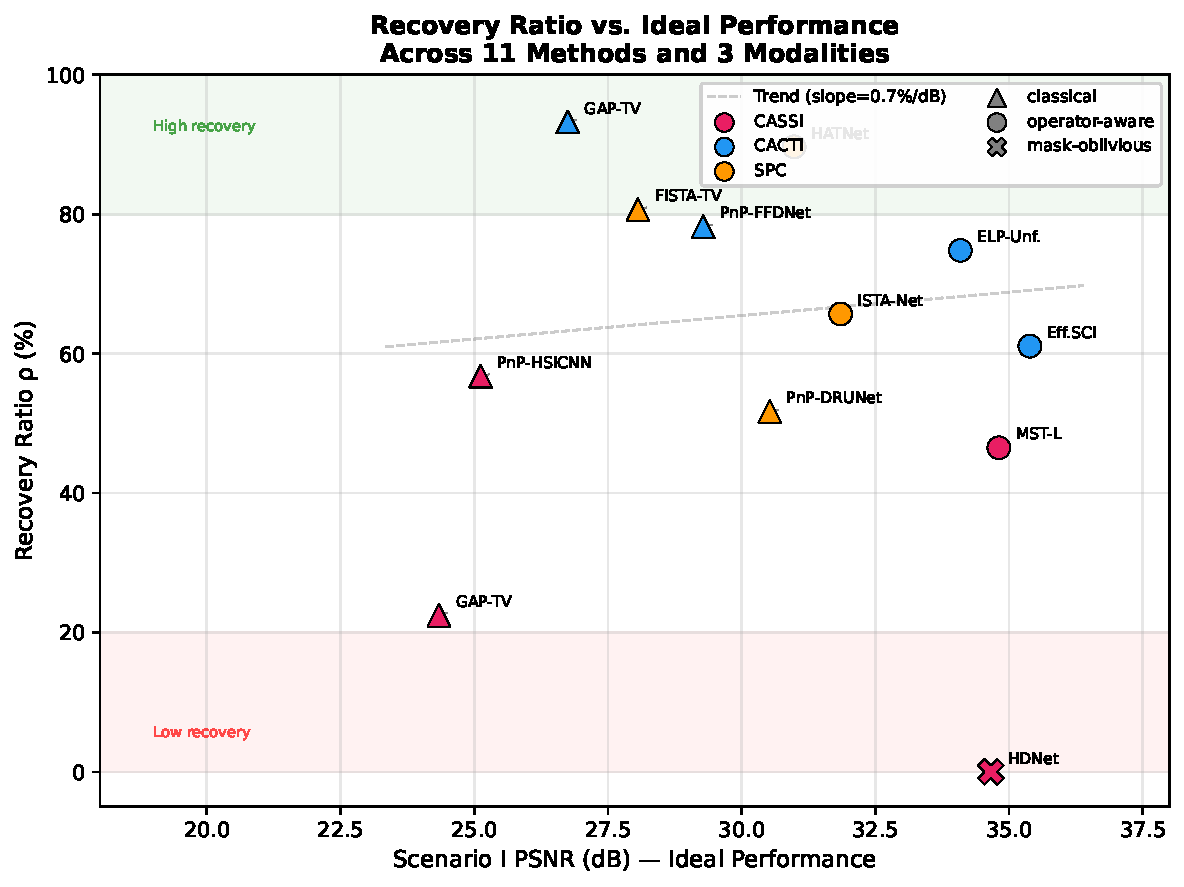
\includegraphics[width=0.75\textwidth]{figures/rho_scatter.pdf}
\caption{Recovery ratio ($\rho$) vs.\ ideal PSNR (Scenario~I) for all 12 methods across three modalities. Color indicates modality; shape indicates method type (classical, operator-aware, mask-oblivious). An inverse trend is visible: higher-performing methods tend to have lower recovery ratios, suggesting that stronger learned priors create greater operator dependence.}
\label{fig:rho_scatter}
\end{figure}

\paragraph{Mismatch severity ranking.}
CACTI suffers the most severe degradation (.54--.67 SSIM drop), driven by its 8-parameter mismatch space where spatial, temporal, and radiometric errors compound.
CASSI's 5-parameter model produces up to .23 SSIM degradation, with dispersion parameters ($a_1$, $\alpha$) creating cumulative sub-pixel shifts across spectral bands.
SPC shows .20--.48 SSIM degradation from gain drift alone.

\paragraph{Recovery potential and architectural patterns.}
\Cref{fig:rho_scatter} visualizes recovery ratio versus ideal performance.
Best recovery varies by modality: ELP-Unfolding achieves 94.2\% on CACTI, HATNet 80.1\% on SPC, PnP-HSICNN 69.6\% on CASSI---the lower CASSI value reflects that current architectures cannot adapt to sub-pixel dispersion drift even with oracle mask knowledge.
Across modalities, a consistent three-way pattern emerges: (i)~classical methods show moderate degradation with high recovery; (ii)~operator-conditioned deep methods show high degradation but substantial recovery; (iii)~mask-oblivious methods show zero recovery.
This taxonomy guides method selection based on calibration availability.

\subsection{Real Hardware Validation}
\label{sec:real_data}

A key limitation of simulation-only benchmarks is uncertainty about whether findings transfer to physical hardware.
We validate InverseNet's simulation patterns on real CASSI and CACTI data.
Full methodological details---including dataset provenance, evaluation metric definitions, per-scene results, and a simulation-vs-real comparison table---are provided in the supplementary material.

\paragraph{CASSI real data.}
We use the TSA real dataset~\cite{choi2017kaist}: 5 real scenes captured on a DD-CASSI prototype with a $660 \times 660$ coded aperture mask and 28 spectral bands (450--650\,nm).
Measurements are $660 \times 714$ detector images.
Since \textbf{no ground truth} exists for real CASSI captures (the true spectral cube cannot be independently measured), we use the normalised measurement residual $r = \|\mathbf{y} - \mathbf{\Phi}_{\text{cal}}\hat{\mathbf{x}}\|^2 / \|\mathbf{y}\|^2$, always evaluated with the \emph{calibrated} mask regardless of which mask was used for reconstruction (see supplementary for why this ``cross-residual'' is essential).
We restrict evaluation to classical and PnP methods.
Deep learning methods (HDNet, MST-L) are excluded because their mask-conditioned reconstructions are produced by fixed pretrained weights; when the input mask changes, the network output changes in a nonlinear, architecture-dependent way that the measurement residual does not disambiguate from signal reconstruction quality.
In other words, $r$ increases for classical methods because they \emph{explicitly} re-fit the forward model each iteration; for deep networks the residual conflates model mismatch with reconstruction artefacts introduced by out-of-distribution inputs.
Evaluating deep networks on real hardware in a principled way requires either paired captures or a task-specific proxy metric; we leave this to future work.
We evaluate two conditions: \emph{calibrated} (hardware mask as-is) and \emph{mismatched} (mask shifted by $dx{=}0.5$, $dy{=}0.3$\,pixels).
\Cref{tab:cassi_real} shows the results.

\begin{table}[t]
\centering
\caption{CASSI real data (5 scenes, $660 \times 660 \times 28$). Normalised measurement residual $r = \|\mathbf{y} - \mathbf{\Phi}_{\text{cal}}\hat{\mathbf{x}}\|^2 / \|\mathbf{y}\|^2$ (lower is better; no ground truth required). Ratio: mismatched\,/\,calibrated. Only classical/PnP methods evaluated (no ground truth for deep learning supervision).}
\label{tab:cassi_real}
\begin{tabular}{@{}lccc@{}}
\toprule
\textbf{Method} & \textbf{Calibrated} & \textbf{Mismatched} & \textbf{Ratio} \\
\midrule
GAP-TV            & 0.0019 & 0.0033 & 1.8$\times$ \\
PnP-HSICNN        & 0.0127 & 0.0142 & 1.1$\times$ \\
\bottomrule
\end{tabular}
\end{table}

Both mask-aware iterative methods (GAP-TV and PnP-HSICNN) show residual increases under mismatch, because they explicitly fit the forward model during reconstruction: when reconstructed with a wrong mask, the result is inconsistent with the true measurement.
GAP-TV shows a modest $1.8\times$ increase, while PnP-HSICNN shows only $1.1\times$---the deep denoiser regularises the reconstruction enough to partially mask the forward-model inconsistency.
This contrasts sharply with CACTI (\cref{sec:cacti_real_data} below), where residuals increase $9.4$--$11.0\times$ under the same spatial shift.

By contrast, our \emph{simulation} experiments (\cref{tab:cassi}) show 3--14\,dB PSNR degradation because they include dispersion perturbation ($a_1$, $\alpha$)---which the real-data experiment does not.
The modest $1.8\times$ residual increase from spatial shift alone (vs.\ $10\times$ for CACTI) validates that \textbf{dispersion mismatch, not spatial shift, is the dominant CASSI degradation source} (\cref{fig:cassi_real}).

\begin{figure}[t]
\centering
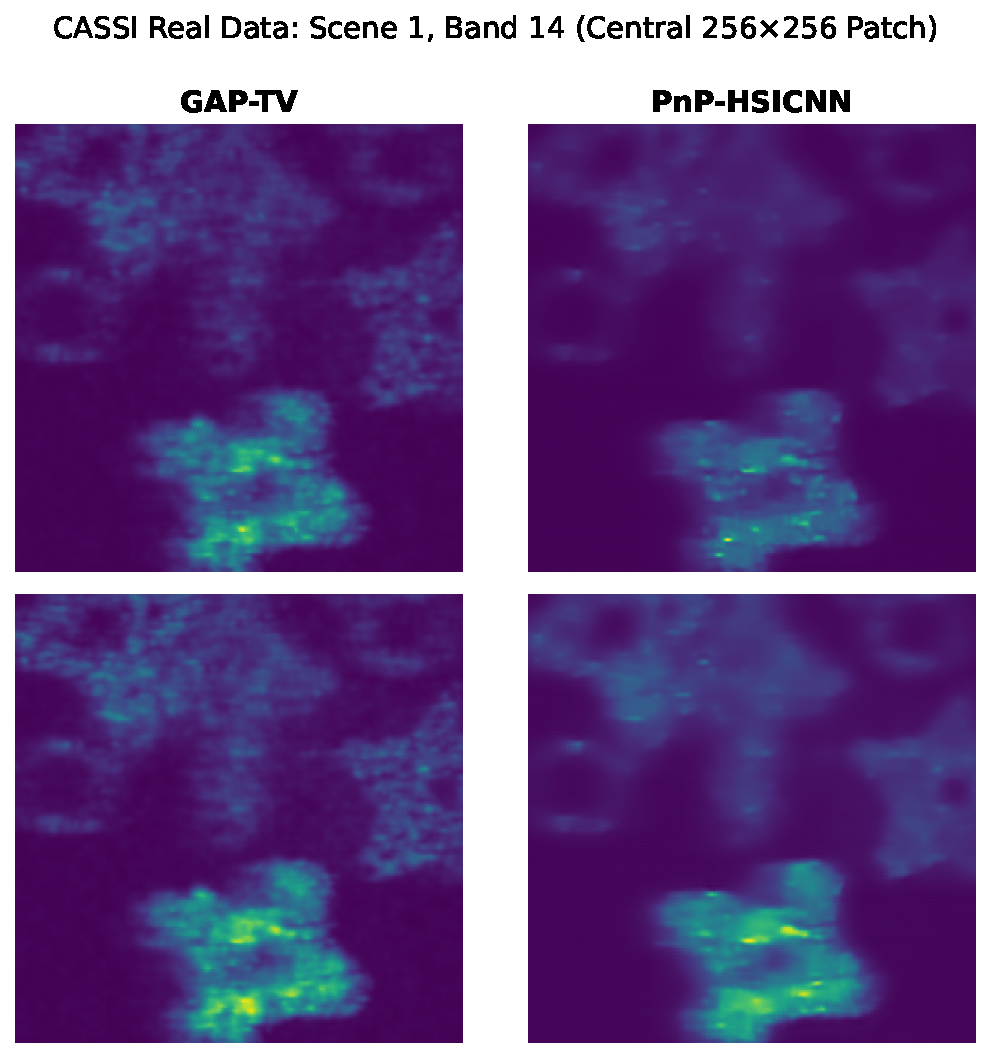
\includegraphics[width=\textwidth]{figures/cassi_real_comparison.pdf}
\caption{CASSI real data (Scene~1, band~14): calibrated (top) vs.\ mismatched (bottom) reconstructions for GAP-TV and PnP-HSICNN. The visual differences are subtle, consistent with the modest residual ratios in \cref{tab:cassi_real}---spatial mask shift alone is not the dominant degradation source for CASSI.}
\label{fig:cassi_real}
\end{figure}

\paragraph{CACTI real data.}
\label{sec:cacti_real_data}
We evaluate 4 real CACTI scenes from the EfficientSCI dataset (cr$=$10), using the same measurement residual metric (no ground truth).
\Cref{tab:cacti_real} shows the results.
Under mask mismatch, GAP-TV residuals increase $9.4$--$11.0\times$, confirming mismatch severely degrades real data fidelity.
PnP-FFDNet shows increases of $1.3$--$2.8\times$ (mean $2.0\times$), higher than GAP-TV's baseline but moderated by FFDNet's learned denoiser.
The large difference in absolute calibrated residuals between GAP-TV (1.6e-5) and PnP-FFDNet (0.0041) reflects their different reconstruction mechanisms: GAP-TV minimises the measurement residual directly as its optimisation objective, so the calibrated residual is near-zero by construction; PnP-FFDNet's outer loop is moderated by the denoiser prior, which prevents full data fidelity and results in a higher but still consistent baseline residual.
The \emph{ratio} (mismatched\,/\,calibrated) is therefore the appropriate comparison metric, not the absolute values.
Mismatched reconstructions exhibit temporal ghosting (\cref{fig:cacti_real}).

\begin{table}[t]
\centering
\caption{CACTI real data (4 scenes, $512 \times 512$, cr$=$10). Normalised measurement residual (lower is better). Ratio: mismatched\,/\,calibrated.}
\label{tab:cacti_real}
\begin{tabular}{@{}lccc@{}}
\toprule
\textbf{Method} & \textbf{Calibrated} & \textbf{Mismatched} & \textbf{Ratio} \\
\midrule
GAP-TV     & 1.6e-5 & 1.6e-4 & 10.4$\times$ \\
PnP-FFDNet & 0.0041 & 0.0069 & 2.0$\times$ \\
\bottomrule
\end{tabular}
\end{table}

\begin{figure}[t]
\centering
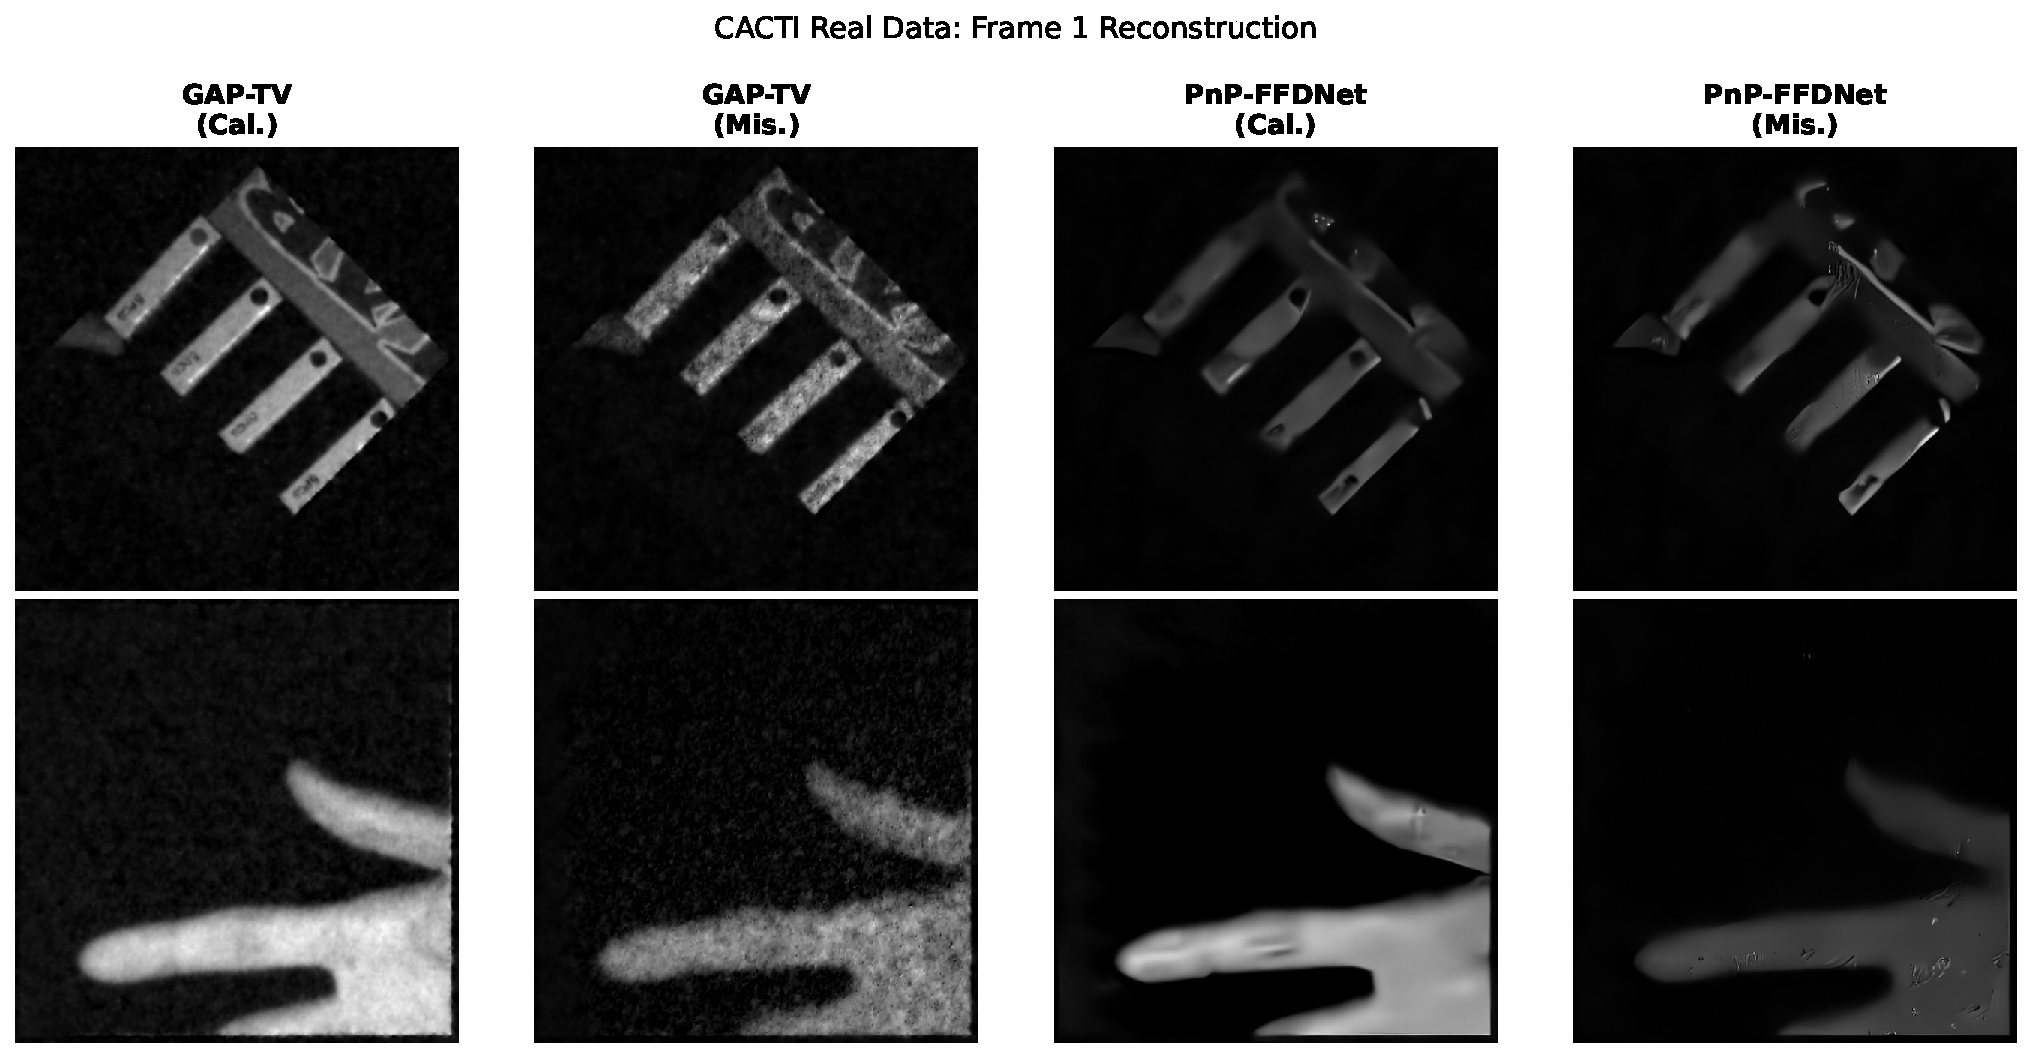
\includegraphics[width=0.9\textwidth]{figures/cacti_real_comparison.pdf}
\caption{CACTI real data: calibrated vs.\ mismatched reconstruction for \textit{duomino} and \textit{hand} scenes. Mismatched masks produce temporal ghosting artifacts, mirroring simulation findings.}
\label{fig:cacti_real}
\end{figure}

\subsection{Scenario~IV: Blind Calibration Baseline}
\label{sec:scenario_iv}

Scenario~III assumes oracle knowledge of the true operator.
In practice, the mismatch parameters must be estimated from measurements alone.
Scenario~IV evaluates blind calibration via grid search over mismatch parameters.
For \emph{geometric} mismatch (CASSI, CACTI), the measurement residual provides a strong calibration signal:
\begin{equation}
    \tilde{\boldsymbol{\theta}} = \arg\min_{\boldsymbol{\theta}} \left\| \mathbf{y} - \mathbf{\Phi}(\boldsymbol{\theta})\, \hat{\mathbf{x}}\!\left(\mathbf{y}, \mathbf{\Phi}(\boldsymbol{\theta})\right) \right\|^2,
    \label{eq:scenario_iv}
\end{equation}
where $\boldsymbol{\theta}$ denotes the mismatch parameters and $\hat{\mathbf{x}}(\mathbf{y}, \mathbf{\Phi})$ is the reconstruction from a fast inner-loop solver.
For \emph{radiometric} mismatch (SPC gain drift), the measurement residual is uninformative because the underdetermined system always achieves near-zero self-consistent residual regardless of gain.
Instead, we use reconstruction sparsity (total variation) as the objective:
\begin{equation}
    \tilde{\alpha} = \arg\min_{\alpha} \mathrm{TV}\!\left(\hat{\mathbf{x}}\!\left(\mathbf{y},\, \mathbf{\Phi}(\alpha)\right)\right),
    \label{eq:scenario_iv_tv}
\end{equation}
where $\mathrm{TV}(\cdot)$ denotes the anisotropic total variation.
The rationale is that the correctly calibrated gain produces a clean corrected measurement, yielding a smooth natural-image reconstruction with low TV; incorrect gain leaves systematic artifacts that increase TV.
No ground truth is required for either criterion.

\paragraph{Procedure.}
For each candidate $\boldsymbol{\theta}$, we: (1)~construct the trial operator $\mathbf{\Phi}(\boldsymbol{\theta})$, (2)~reconstruct $\hat{\mathbf{x}}$ using a fast classical solver, and (3)~evaluate the objective (measurement residual for CASSI/CACTI, TV for SPC).
The parameter yielding the lowest objective is selected, and a final high-quality reconstruction is performed with that operator.
Calibration uses a subset of the data: 3 KAIST scenes for CASSI, 2 benchmark videos for CACTI, and 2 Set11 images for SPC---all from the same datasets as \cref{sec:cassi,sec:cacti,sec:spc}, with the same mismatch parameters.

\paragraph{CASSI and CACTI results.}
For CACTI, grid search over mask shifts $dx, dy \in [-1.0, 1.0]$\,px ($9 \times 9$ grid) achieves \emph{near-perfect} calibration: 26.99\,dB (matching Scenario~III), recovering the full 9.39\,dB mismatch gap.
\emph{Important scope caveat}: this grid search calibrates only 2 of the 8 CACTI mismatch parameters ($dx$ and $dy$); the remaining 6 parameters (rotation $\theta$, temporal offset $\Delta t$, duty cycle $\eta$, gain $g$, offset $o$, noise $\sigma_n$) are held at their ground-truth values during calibration. The result therefore measures the upper bound of what 2-parameter spatial calibration can achieve, not full 8-parameter recovery. Extending to the full mismatch space is left to future work.
For CASSI ($11 \times 11$ grid over $dx, dy$), calibration recovers 85\% of the spatial gap ($+1.44$\,dB of $+1.69$\,dB possible); the residual 15\% reflects spatial estimation error ($\hat{dx}{=}0.4$ vs.\ true $0.5$\,px).
The measurement residual provides a strong signal for geometric mismatch because mask shifts cause large, structured data inconsistencies.

\paragraph{SPC results.}
\Cref{tab:spc_scenario_iv} shows the SPC calibration results using TV minimisation (\cref{eq:scenario_iv_tv}).
Grid search over $\alpha \in [0, 0.005]$ with 41 points ($33 \times 33$ blocks, ISTA-Net's learned $\mathbf{\Phi}$) estimates $\hat{\alpha} = 0.00125$ vs.\ true $\alpha = 0.0015$ for both methods, recovering 86--92\% of the oracle bound.
The TV surface exhibits a clear bowl-shaped minimum near the true $\alpha$, confirming that reconstruction sparsity is a viable calibration objective for radiometric mismatch.
PnP-DRUNet achieves higher recovery (92\%) than FISTA-TV (86\%) because the learned denoiser prior produces sharper reconstructions whose TV is more sensitive to residual gain artifacts.
This contrasts with the measurement residual, which is flat across all $\alpha$ values for SPC (the underdetermined system can always self-consistently fit any gain-corrected measurements).

\begin{table}[t]
\centering
\caption{SPC blind calibration via TV minimisation (\cref{eq:scenario_iv_tv}). II: mismatched, no calibration. IV: estimated $\hat{\alpha}$ via TV grid search. III: oracle (true $\alpha$). Recovery: (IV$-$II)\,/\,(III$-$II). True $\alpha{=}0.0015$; estimated $\hat{\alpha}{=}0.00125$.}
\label{tab:spc_scenario_iv}
\begin{tabular}{@{}lcccc@{}}
\toprule
\textbf{Method} & \textbf{II} & \textbf{IV} & \textbf{III} & \textbf{Recovery} \\
\midrule
FISTA-TV   & 19.78 & 26.54 & 27.60 & 86\% \\
PnP-DRUNet & 18.34 & 25.39 & 26.01 & 92\% \\
\bottomrule
\end{tabular}
\end{table}

\paragraph{Criterion comparison.}
The geometric/radiometric distinction reveals that blind calibration requires \emph{matching the objective to the mismatch type}: measurement residual for geometric mismatch (where operator errors create large data infidelities), and reconstruction sparsity for radiometric mismatch (where the operator structure is preserved but measurement values are scaled).
Across all three modalities, Scenario~IV recovers 85--100\% of the oracle bound, demonstrating that blind calibration is practical for all mismatch types studied.

% ============================================================================
% 5. DISCUSSION
% ============================================================================
\section{Discussion}
\label{sec:discussion}

\paragraph{Classical vs.\ deep learning robustness.}
Classical methods are consistently more robust: GAP-TV loses 3.38\,dB on CASSI and 10.94\,dB on CACTI, vs.\ 13.98\,dB and 20.58\,dB for the best deep networks.
Under mismatch, the performance hierarchy \emph{inverts}: on CACTI Scenario~II, GAP-TV (15.81\,dB) outperforms EfficientSCI (14.81\,dB) despite being 8.64\,dB worse under ideal conditions---confirming that physical model fidelity dominates algorithmic sophistication.

\paragraph{The operator-awareness spectrum.}
Methods exist on a spectrum: \emph{mask-oblivious} (HDNet, $\rho{=}0\%$) cannot benefit from calibration; \emph{operator-conditioned} (MST, HATNet, $\rho{=}41$--$90\%$) achieve high calibration gains but suffer the largest degradation; \emph{operator-iterative} (GAP-TV, FISTA-TV, $\rho{=}81$--$93\%$ on CACTI/SPC) use the operator directly in each iteration.
This taxonomy reframes the problem: the critical bottleneck is not algorithmic sophistication but \emph{physical model fidelity}.

\paragraph{Practical implications.}
When recalibration is feasible, operator-conditioned networks should be paired with Scenario~IV-style calibration.
When calibration is impractical, classical methods provide the most robust baseline, with degradation 3--5$\times$ smaller than deep methods.
Scenario~IV demonstrates that simple grid-search calibration recovers 85--100\% of the oracle bound without ground truth, provided the objective matches the mismatch type: measurement residual for geometric mismatch, reconstruction sparsity for radiometric mismatch.

\paragraph{Limitations.}
Our parametric mismatch models (affine shifts, gain drift) capture dominant error sources but do not cover spatially varying PSF errors or nonlinear detector response.
Real hardware validation covers CASSI and CACTI; SPC real data would strengthen generalisability.
The grid-search calibration does not scale to high-dimensional spaces---gradient-based or learned calibration is a natural next step.
The benchmark currently evaluates 4 methods per modality; expanding to include recent advances (DAUHST~\cite{cai2022dauhst}, CST~\cite{cai2022cst}, DiffSCI~\cite{meng2024diffsci}) would broaden coverage and further validate the observed trends.
The within-modality inverse performance--robustness relationship is observed over $N{=}4$ methods; cross-modality pooling (12 methods total, Spearman $r_s{=}{-}0.71$) provides stronger statistical support but future work should increase per-modality sample size.

\paragraph{Residual gap analysis.}
The residual gap $\Delta_{\text{res}} = \text{PSNR}_{\text{I}} - \text{PSNR}_{\text{III}}$ measures unrecoverable losses.
CASSI shows the largest residual gaps (MST-L: 7.48\,dB) due to fixed-step dispersion assumptions, while CACTI (GAP-TV: 0.74\,dB) and SPC (HATNet: 1.20\,dB) confirm that spatial and gain-type mismatches are nearly fully recoverable.
Per-method residual gap visualizations are provided in the supplementary material.

% ============================================================================
% 6. CONCLUSION
% ============================================================================
\section{Conclusion}
\label{sec:conclusion}

We have presented InverseNet, the first cross-modality benchmark for operator mismatch in compressive imaging.
Evaluating 12 methods across CASSI, CACTI, and SPC under a four-scenario protocol, we find:
(1)~mismatch degrades deep learning methods by 10--21\,dB, collapsing their advantage over classical methods;
(2)~operator-conditioned architectures recover 40--90\% of losses through calibration, while mask-oblivious ones recover 0\%;
(3)~blind grid-search calibration (Scenario~IV) recovers 85--100\% of the oracle bound without ground truth, using measurement residual for geometric and reconstruction sparsity for radiometric mismatch;
(4)~real hardware experiments confirm simulation patterns transfer to physical data.
When calibration is feasible, operator-conditioned networks paired with self-supervised calibration are optimal; otherwise, classical methods provide the most robust baseline.

All reconstruction arrays, metrics, and code will be released upon acceptance.
Future work includes gradient-based calibration, dispersion-aware architectures, and expansion to lensless imaging and ptychography.

\paragraph{Data availability.}
All test data used in this work come from existing public datasets: KAIST~\cite{choi2017kaist} for CASSI, the CACTI benchmark~\cite{yuan2021snapshot}, and Set11~\cite{kulkarni2016reconnet} for SPC. Real CASSI scenes are from the TSA dataset~\cite{wagadarikar2008cassi}; real CACTI scenes are from the EfficientSCI repository~\cite{wang2023efficientsci}. No non-public datasets were used. Code and reconstruction arrays are available at \url{https://github.com/integritynoble/Physics_World_Model}.

% ============================================================================
% REFERENCES
% ============================================================================
\bibliographystyle{splncs04}
\begin{thebibliography}{99}

\bibitem{wagadarikar2008cassi}
Wagadarikar, A., John, R., Willett, R., Brady, D.:
Single disperser design for coded aperture snapshot spectral imaging.
Applied Optics \textbf{47}(10), B44--B51 (2008)

\bibitem{meng2020e2e}
Meng, Z., Ma, J., Yuan, X.:
End-to-end low cost compressive spectral imaging with spatial-spectral self-attention.
In: ECCV. pp.~187--204 (2020)

\bibitem{llull2013cacti}
Llull, P., Liao, X., Yuan, X., Yang, J., Kittle, D., Carin, L., Sapiro, G., Brady, D.J.:
Coded aperture compressive temporal imaging.
Optics Express \textbf{21}(9), 10526--10545 (2013)

\bibitem{yuan2021snapshot}
Yuan, X., Brady, D.J., Katsaggelos, A.K.:
Snapshot compressive imaging: Theory, algorithms, and applications.
IEEE Signal Processing Magazine \textbf{38}(2), 65--88 (2021)

\bibitem{duarte2008spc}
Duarte, M.F., Davenport, M.A., Takhar, D., Laska, J.N., Sun, T., Kelly, K.F., Baraniuk, R.G.:
Single-pixel imaging via compressive sampling.
IEEE Signal Processing Magazine \textbf{25}(2), 83--91 (2008)

\bibitem{edgar2019spc_review}
Edgar, M.P., Gibson, G.M., Padgett, M.J.:
Principles and prospects for single-pixel imaging.
Nature Photonics \textbf{13}(1), 13--20 (2019)

\bibitem{yuan2016gaptv}
Yuan, X.:
Generalized alternating projection based total variation minimization for compressive sensing.
In: ICIP. pp.~2539--2543 (2016)

\bibitem{beck2009fista}
Beck, A., Teboulle, M.:
A fast iterative shrinkage-thresholding algorithm for linear inverse problems.
SIAM Journal on Imaging Sciences \textbf{2}(1), 183--202 (2009)

\bibitem{boyd2011admm}
Boyd, S., Parikh, N., Chu, E., Peleato, B., Eckstein, J.:
Distributed optimization and statistical learning via the alternating direction method of multipliers.
Foundations and Trends in Machine Learning \textbf{3}(1), 1--122 (2011)

\bibitem{cai2022mst}
Cai, Y., Lin, J., Hu, X., Wang, H., Yuan, X., Zhang, Y., Timofte, R., Van Gool, L.:
Mask-guided spectral-wise transformer for efficient hyperspectral image reconstruction.
In: CVPR. pp.~17502--17511 (2022)

\bibitem{hu2022hdnet}
Hu, X., Cai, Y., Lin, J., Wang, H., Yuan, X., Zhang, Y., Timofte, R., Van Gool, L.:
HDNet: High-resolution dual-domain learning for spectral compressive imaging.
In: CVPR. pp.~17542--17551 (2022)

\bibitem{wang2023efficientsci}
Wang, L., Cao, M., Yuan, X.:
EfficientSCI: Densely connected network with space-time factorization for large-scale video snapshot compressive imaging.
In: CVPR. pp.~18477--18486 (2023)

\bibitem{yang2022elp}
Yang, C., Zhang, S., Yuan, X.:
Ensemble learning priors driven deep unfolding for scalable video snapshot compressive imaging.
In: ECCV. pp.~600--618 (2022)

\bibitem{zhang2018istanet}
Zhang, J., Ghanem, B.:
ISTA-Net: Interpretable optimization-inspired deep network for image compressive sensing.
In: CVPR. pp.~1828--1837 (2018)

\bibitem{qu2024hatnet}
Qu, G., Wang, P., Yuan, X.:
Dual-scale transformer for large-scale single-pixel imaging.
In: CVPR. pp.~25327--25337 (2024)

\bibitem{yuan2020pnp}
Yuan, X., Liu, Y., Suo, J., Dai, Q.:
Plug-and-play algorithms for large-scale snapshot compressive imaging.
In: CVPR. pp.~1447--1457 (2020)

\bibitem{choi2017kaist}
Choi, I., Jeon, D.S., Nam, G., Gutierrez, D., Kim, M.H.:
High-quality hyperspectral reconstruction using a spectral prior.
ACM Transactions on Graphics \textbf{36}(6), 218:1--218:13 (2017)

\bibitem{kulkarni2016reconnet}
Kulkarni, K., Lohit, S., Turaga, P., Kerviche, R., Ashok, A.:
ReconNet: Non-iterative reconstruction of images from compressively sensed measurements.
In: CVPR. pp.~449--458 (2016)

\bibitem{zbontar2018fastmri}
Zbontar, J., Knoll, F., Sriram, A., Murrell, T., Huang, Z., Muckley, M.J., Defazio, A., Stern, R., Johnson, P., Bruno, M., et~al.:
fastMRI: An open dataset and benchmarks for accelerated MRI.
arXiv preprint arXiv:1811.08839 (2018)


\bibitem{arguello2013cassi_calib}
Arguello, H., Rueda, H., Wu, Y., Prather, D.W., Arce, G.R.:
Higher-order computational model for coded aperture spectral imaging.
Applied Optics \textbf{52}(10), D12--D21 (2013)

\bibitem{wang2004ssim}
Wang, Z., Bovik, A.C., Sheikh, H.R., Simoncelli, E.P.:
Image quality assessment: from error visibility to structural similarity.
IEEE Transactions on Image Processing \textbf{13}(4), 600--612 (2004)

\bibitem{cai2022dauhst}
Cai, Y., Lin, J., Wang, H., Yuan, X., Ding, H., Zhang, Y., Timofte, R., Van Gool, L.:
Degradation-aware unfolding half-shuffle transformer for spectral compressive imaging.
In: NeurIPS (2022)

\bibitem{cai2022cst}
Cai, Y., Lin, J., Hu, X., Wang, H., Yuan, X., Zhang, Y., Timofte, R., Van Gool, L.:
Coarse-to-fine sparse transformer for hyperspectral image reconstruction.
In: ECCV. pp.~686--704 (2022)


\bibitem{adler2018learned}
Adler, J., {\"O}ktem, O.:
Learned primal-dual reconstruction.
IEEE Transactions on Medical Imaging \textbf{37}(6), 1322--1332 (2018)

\bibitem{ryu2019pnp}
Ryu, E., Liu, J., Wang, S., Chen, X., Wang, Z., Yin, W.:
Plug-and-play methods provably converge with properly trained denoisers.
In: ICML. pp.~5546--5557 (2019)

\bibitem{moult2005casp}
Moult, J., Fidelis, K., Zemla, A., Hubbard, T.:
Critical assessment of methods of protein structure prediction (CASP)---round 6.
Proteins \textbf{61}(S7), 3--7 (2005)


\bibitem{antun2020instabilities}
Antun, V., Renna, F., Poon, C., Adcock, B., Hansen, A.C.:
On instabilities of deep learning in image reconstruction and the potential costs of AI.
PNAS \textbf{117}(48), 30088--30098 (2020)

\bibitem{timofte2017ntire}
Timofte, R., Agustsson, E., Van Gool, L., et al.:
NTIRE 2017 challenge on single image super-resolution: Methods and results.
In: CVPR Workshops. pp.~1110--1121 (2017)

\bibitem{kohler2020super}
K{\"o}hler, T., B{\"a}tz, M., Naderi, F., et al.:
Toward bridging the simulated-to-real gap: Benchmarking super-resolution on real data.
IEEE TPAMI \textbf{42}(11), 2944--2959 (2020)

\bibitem{li2023rdluf}
Li, Y., Cai, Y., Lin, J., Hu, X., Yuan, X., Zhang, Y., Timofte, R., Van Gool, L.:
RDLUF-MixS$^2$: Spatial-spectral feature mixing for spectral compressive imaging.
In: CVPR. pp.~22262--22271 (2023)

\bibitem{meng2024diffsci}
Meng, Z., Yu, Z., Xu, K., Yuan, X.:
DiffSCI: Zero-shot snapshot compressive imaging via iterative spectral diffusion model.
In: CVPR. pp.~25857--25867 (2024)

\bibitem{berk2024robust}
Berk, A., Plan, Y., Bhatt, N.:
Robustness of compressed sensing under structured model mismatch.
Foundations of Computational Mathematics \textbf{24}(4), 1285--1337 (2024)


\bibitem{zheng2021pnp}
Zheng, S., Liu, Y., Meng, Z., M{\"u}ller, M., Shu, R., Yuan, X.:
Deep plug-and-play priors for spectral snapshot compressive imaging.
Photonics Research \textbf{9}(2), B18--B29 (2021)

\bibitem{zhang2021drunet}
Zhang, K., Li, Y., Zuo, W., Zhang, L., Van Gool, L., Timofte, R.:
Plug-and-play image restoration with deep denoiser prior.
IEEE Transactions on Pattern Analysis and Machine Intelligence \textbf{44}(10), 6360--6376 (2022)

\end{thebibliography}

\appendix

\maketitle

% ============================================================================
% A. PER-SCENE RESULTS
% ============================================================================
\section{Per-Scene Detailed Results}
\label{sec:per_scene}

\subsection{CASSI Per-Scene PSNR}

\Cref{tab:cassi_perscene} reports per-scene PSNR for all four CASSI methods across three scenarios, along with per-scene recovery ratios.

\begin{table}[h]
\centering
\caption{CASSI per-scene PSNR (dB) and recovery ratio $\rho$ (\%). 10 KAIST scenes, $256 \times 256 \times 28$. 5-parameter mismatch ($dx{=}0.5$\,px, $dy{=}0.3$\,px, $\theta{=}0.1^\circ$, $a_1{=}2.02$, $\alpha{=}0.15^\circ$).}
\label{tab:cassi_perscene}
\resizebox{\textwidth}{!}{%
\begin{tabular}{@{}l|ccc|c|ccc|c|ccc|c|ccc|c@{}}
\toprule
& \multicolumn{4}{c|}{\textbf{GAP-TV}} & \multicolumn{4}{c|}{\textbf{PnP-HSICNN}} & \multicolumn{4}{c|}{\textbf{HDNet}} & \multicolumn{4}{c}{\textbf{MST-L}} \\
\textbf{Scene} & \textbf{I} & \textbf{II} & \textbf{III} & $\boldsymbol{\rho}$ & \textbf{I} & \textbf{II} & \textbf{III} & $\boldsymbol{\rho}$ & \textbf{I} & \textbf{II} & \textbf{III} & $\boldsymbol{\rho}$ & \textbf{I} & \textbf{II} & \textbf{III} & $\boldsymbol{\rho}$ \\
\midrule
Scene 1  & 26.49 & 24.08 & 24.18 & 4.1\% & 27.43 & 23.47 & 25.78 & 58.3\% & 34.95 & 24.37 & 24.37 & 0.0\% & 35.29 & 23.96 & 29.98 & 53.2\% \\
Scene 2  & 24.60 & 21.89 & 22.82 & 34.5\% & 25.34 & 21.56 & 23.80 & 59.3\% & 35.65 & 23.26 & 23.26 & 0.0\% & 36.14 & 22.21 & 28.42 & 44.6\% \\
Scene 3  & 25.96 & 18.62 & 19.68 & 14.4\% & 26.71 & 17.59 & 21.83 & 46.5\% & 35.54 & 18.61 & 18.61 & 0.0\% & 35.66 & 16.09 & 23.57 & 38.2\% \\
Scene 4  & 28.36 & 23.37 & 24.41 & 20.9\% & 28.80 & 22.89 & 25.98 & 52.3\% & 41.63 & 23.98 & 23.98 & 0.0\% & 40.05 & 21.91 & 29.80 & 43.5\% \\
Scene 5  & 23.66 & 20.39 & 21.27 & 26.9\% & 24.65 & 19.36 & 22.75 & 64.3\% & 32.56 & 20.22 & 20.22 & 0.0\% & 32.84 & 20.28 & 26.75 & 51.5\% \\
Scene 6  & 22.34 & 20.39 & 21.00 & 31.2\% & 23.12 & 20.29 & 21.80 & 53.0\% & 34.33 & 22.63 & 22.63 & 0.0\% & 34.56 & 22.37 & 28.67 & 51.7\% \\
Scene 7  & 23.51 & 20.56 & 21.07 & 17.4\% & 24.94 & 19.86 & 22.77 & 57.4\% & 33.27 & 20.79 & 20.79 & 0.0\% & 33.80 & 19.76 & 26.12 & 45.3\% \\
Scene 8  & 22.16 & 20.57 & 21.10 & 33.3\% & 22.73 & 20.30 & 21.92 & 66.4\% & 32.26 & 22.73 & 22.73 & 0.0\% & 32.74 & 21.33 & 27.44 & 53.5\% \\
Scene 9  & 23.03 & 19.14 & 20.61 & 37.8\% & 24.03 & 18.79 & 21.82 & 57.8\% & 34.18 & 21.18 & 21.18 & 0.0\% & 34.37 & 19.75 & 26.71 & 47.6\% \\
Scene 10 & 23.27 & 20.58 & 21.04 & 16.9\% & 23.47 & 19.90 & 22.38 & 69.4\% & 32.22 & 21.06 & 21.06 & 0.0\% & 32.63 & 20.69 & 25.86 & 43.3\% \\
\midrule
\textbf{Mean} & 24.34 & 20.96 & 21.72 & 22.5\% & 25.12 & 20.40 & 23.08 & \best{56.8\%} & 34.66 & 21.88 & 21.88 & 0.0\% & 34.81 & 20.83 & 27.33 & 46.5\% \\
\bottomrule
\end{tabular}%
}
\end{table}

\subsection{CACTI Per-Video PSNR}

\Cref{tab:cacti_pervideo} reports per-video PSNR for all four CACTI methods.

\begin{table}[h]
\centering
\caption{CACTI per-video PSNR (dB) and recovery ratio $\rho$ (\%). 6 benchmark videos, $256 \times 256 \times 8$. 8-parameter mismatch.}
\label{tab:cacti_pervideo}
\resizebox{\textwidth}{!}{%
\begin{tabular}{@{}l|ccc|c|ccc|c|ccc|c|ccc|c@{}}
\toprule
& \multicolumn{4}{c|}{\textbf{GAP-TV}} & \multicolumn{4}{c|}{\textbf{PnP-FFDNet}} & \multicolumn{4}{c|}{\textbf{ELP-Unfolding}} & \multicolumn{4}{c}{\textbf{EfficientSCI}} \\
\textbf{Video} & \textbf{I} & \textbf{II} & \textbf{III} & $\boldsymbol{\rho}$ & \textbf{I} & \textbf{II} & \textbf{III} & $\boldsymbol{\rho}$ & \textbf{I} & \textbf{II} & \textbf{III} & $\boldsymbol{\rho}$ & \textbf{I} & \textbf{II} & \textbf{III} & $\boldsymbol{\rho}$ \\
\midrule
Kobe    & 26.70 & 18.97 & 26.50 & 97.4\% & 30.02 & 16.00 & 29.20 & 94.2\% & 34.07 & 18.31 & 32.63 & 90.9\% & 35.55 & 18.21 & 32.43 & 82.0\% \\
Traffic & 20.73 & 13.99 & 20.57 & 97.6\% & 24.06 & 9.95  & 23.37 & 95.1\% & 31.33 & 13.90 & 29.04 & 86.8\% & 32.19 & 13.30 & 27.08 & 72.9\% \\
Runner  & 29.34 & 17.70 & 28.85 & 95.8\% & 32.88 & 13.40 & 31.18 & 91.3\% & 38.14 & 17.00 & 34.06 & 80.7\% & 39.28 & 16.65 & 31.15 & 65.5\% \\
Drop    & 34.22 & 13.64 & 31.43 & 86.4\% & 38.71 & 7.55  & 21.91 & 46.1\% & 40.08 & 13.52 & 25.12 & 43.7\% & 42.36 & 11.63 & 21.95 & 33.6\% \\
Crash   & 24.80 & 14.77 & 24.45 & 96.5\% & 24.81 & 10.11 & 23.32 & 89.9\% & 29.38 & 14.82 & 26.84 & 82.5\% & 30.62 & 14.25 & 25.07 & 66.1\% \\
Aerial  & 25.22 & 16.76 & 24.95 & 96.8\% & 24.56 & 12.79 & 23.77 & 93.3\% & 30.43 & 16.14 & 28.80 & 88.5\% & 31.24 & 15.92 & 27.18 & 73.5\% \\
\midrule
\textbf{Mean} & 26.75 & 15.81 & 26.01 & \best{93.3\%} & 29.28 & 11.43 & 25.39 & 78.2\% & 34.09 & 15.47 & 29.40 & 74.8\% & 35.39 & 14.81 & 27.38 & 61.1\% \\
\bottomrule
\end{tabular}%
}
\end{table}

\subsection{SPC Per-Image PSNR}

\Cref{tab:spc_perimage} reports per-image PSNR for all four SPC methods.
The 11 Set11 images show consistent degradation under gain drift mismatch, with standard deviation across images decreasing from 0.95--3.38\,dB (Scenario~I) to 0.59--0.69\,dB (Scenario~II), confirming the mismatch-induced performance floor.

\begin{table}[h]
\centering
\caption{SPC per-image PSNR (dB) and recovery ratio $\rho$ (\%). 11 Set11 images, $256 \times 256$, 25\% sampling. Gain drift mismatch ($\alpha{=}0.0015$, $\sigma_y{=}0.03$).}
\label{tab:spc_perimage}
\resizebox{\textwidth}{!}{%
\begin{tabular}{@{}l|ccc|c|ccc|c|ccc|c|ccc|c@{}}
\toprule
& \multicolumn{4}{c|}{\textbf{FISTA-TV}} & \multicolumn{4}{c|}{\textbf{PnP-DRUNet}} & \multicolumn{4}{c|}{\textbf{ISTA-Net}} & \multicolumn{4}{c}{\textbf{HATNet}} \\
\textbf{Image} & \textbf{I} & \textbf{II} & \textbf{III} & $\boldsymbol{\rho}$ & \textbf{I} & \textbf{II} & \textbf{III} & $\boldsymbol{\rho}$ & \textbf{I} & \textbf{II} & \textbf{III} & $\boldsymbol{\rho}$ & \textbf{I} & \textbf{II} & \textbf{III} & $\boldsymbol{\rho}$ \\
\midrule
Monarch     & 28.04 & 19.22 & 26.15 & 78.6\% & 31.43 & 17.25 & 23.77 & 46.0\% & 32.54 & 19.90 & 27.70 & 61.7\% & 30.91 & 20.36 & 29.77 & 89.2\% \\
Parrots     & 27.40 & 18.53 & 26.18 & 86.3\% & 29.85 & 16.18 & 23.15 & 51.0\% & 31.42 & 18.99 & 27.82 & 71.0\% & 31.63 & 19.51 & 30.42 & 90.1\% \\
barbara     & 24.48 & 18.49 & 23.79 & 88.4\% & 28.14 & 16.26 & 22.22 & 50.2\% & 27.84 & 19.02 & 25.53 & 73.7\% & 30.72 & 19.55 & 29.45 & 88.6\% \\
boats       & 28.79 & 18.86 & 26.85 & 80.4\% & 31.57 & 16.47 & 24.25 & 51.5\% & 32.91 & 19.26 & 27.89 & 63.2\% & 31.04 & 19.58 & 29.76 & 88.9\% \\
cameraman   & 26.04 & 18.78 & 24.96 & 85.1\% & 26.48 & 16.69 & 22.49 & 59.2\% & 28.61 & 19.31 & 26.16 & 73.7\% & 29.68 & 19.77 & 28.68 & 89.9\% \\
fingerprint & 23.08 & 17.33 & 22.58 & 91.2\% & 26.36 & 14.75 & 21.05 & 54.3\% & 28.10 & 18.16 & 25.56 & 74.5\% & 30.11 & 18.84 & 29.15 & 91.5\% \\
flinstones  & 24.64 & 17.18 & 23.59 & 86.0\% & 29.25 & 15.33 & 23.16 & 56.3\% & 29.37 & 18.01 & 26.39 & 73.8\% & 29.48 & 18.49 & 28.52 & 91.2\% \\
foreman     & 35.10 & 17.96 & 30.42 & 72.7\% & 36.97 & 15.53 & 26.11 & 49.3\% & 38.23 & 18.20 & 29.68 & 57.3\% & 32.80 & 18.34 & 31.31 & 89.7\% \\
house       & 32.20 & 18.90 & 29.20 & 77.4\% & 35.52 & 16.71 & 25.97 & 49.2\% & 35.70 & 19.23 & 29.21 & 60.6\% & 32.17 & 19.34 & 30.80 & 89.4\% \\
lena256     & 28.97 & 19.25 & 27.13 & 81.1\% & 27.48 & 16.97 & 23.33 & 60.5\% & 32.30 & 19.67 & 27.96 & 65.7\% & 31.22 & 19.96 & 29.89 & 88.2\% \\
peppers256  & 29.95 & 19.11 & 27.51 & 77.5\% & 32.74 & 17.00 & 24.68 & 48.8\% & 33.33 & 19.49 & 28.01 & 61.6\% & 31.05 & 19.68 & 29.87 & 89.6\% \\
\midrule
\textbf{Mean} & 28.06 & 18.51 & 26.21 & 80.7\% & 30.53 & 16.29 & 23.65 & 51.7\% & 31.85 & 19.02 & 27.45 & 65.7\% & 30.98 & 19.40 & 29.78 & \best{89.6\%} \\
\bottomrule
\end{tabular}%
}
\end{table}

% ============================================================================
% A2. REAL HARDWARE VALIDATION: DETAILED METHODOLOGY
% ============================================================================
\section{Real Hardware Validation: Detailed Methodology}
\label{sec:real_perscene}

This section provides full methodological details for the real hardware experiments summarised in Section~4.5 of the main paper.

\subsection{CASSI Real Data}

\subsubsection{Dataset.}
We use the TSA real dataset published by Meng et al.\ (ECCV 2020), which is publicly available in the MST repository.
The dataset provides:
\begin{itemize}
    \item \textbf{5 real measurements}: \texttt{scene1.mat} through \texttt{scene5.mat}, each a $660 \times 714$ detector image captured on a DD-CASSI prototype. These are real photon counts from a physical coded aperture spectral imager.
    \item \textbf{Hardware-calibrated mask}: \texttt{mask.mat}, a $660 \times 660$ binary coded aperture pattern obtained from the physical system's calibration.
    \item \textbf{3D shifted mask}: \texttt{mask\_3d\_shift.mat}, a $660 \times 714 \times 28$ tensor representing the mask after applying the known dispersion pattern ($s{=}2$\,px/band), used directly by deep learning methods.
    \item \textbf{Reference reconstructions} (supplementary use only): \texttt{Recon\_scene1.mat} through \texttt{Recon\_scene5.mat}, each a $660 \times 660 \times 28$ hyperspectral cube reconstructed by the dataset authors. These are \emph{not ground truth}---see below.
\end{itemize}

\subsubsection{Why no PSNR? Evaluation metric choice.}
Real CASSI hardware captures a single 2D measurement from which the 3D spectral cube must be recovered.
There is no independent sensor that captures the true $660 \times 660 \times 28$ spectral cube simultaneously.
Therefore, \textbf{no ground truth exists} for real CASSI data, and \textbf{PSNR cannot be meaningfully computed}.

The dataset does include ``reference reconstructions'' produced by the authors' best algorithm, but these are themselves algorithmic outputs---not physical measurements of the true scene.
Computing PSNR against them would conflate reconstruction quality with similarity to a particular algorithm's output.

Instead, we use the \textbf{normalised measurement residual} as the primary metric (same as CACTI):
\begin{equation}
    r = \frac{\|\mathbf{y} - \sum_{\lambda} M(\cdot, \cdot - d(\lambda)) \cdot \hat{x}(\cdot, \cdot, \lambda)\|^2}{\|\mathbf{y}\|^2}.
\end{equation}
This metric requires \emph{only} the real measurement $\mathbf{y}$ and the calibrated mask $M$---no ground truth.
Crucially, we always evaluate the residual using the \textbf{calibrated} (hardware-provided) mask, regardless of which mask was used for reconstruction.
This ``cross-residual'' measures whether the reconstruction is consistent with the \emph{true} forward model.
Using the reconstruction mask instead (``self-consistent residual'') would be misleading for iterative methods like GAP-TV, which directly minimise the data fidelity term and would trivially achieve low residual even under mismatch.
The diagnostic quantity is the \emph{ratio} of mismatched to calibrated residual: a ratio $\gg 1$ indicates the mismatch damages data fidelity.

For completeness, we also report PSNR against the reference reconstructions in the per-scene table below, but this should be interpreted with caution as it measures similarity to another algorithm's output, not reconstruction accuracy.

\subsubsection{Experimental protocol.}
For each of the 5 real scenes, we run each reconstruction method twice:
\begin{enumerate}
    \item \textbf{Calibrated condition}: use the hardware-provided mask (\texttt{mask.mat} and \texttt{mask\_3d\_shift.mat}) as-is. This represents the best-case scenario where the mask used for reconstruction matches the physical mask in the camera.
    \item \textbf{Mismatched condition}: shift the mask by $dx{=}0.5$\,px, $dy{=}0.3$\,px using bilinear interpolation before reconstruction. This simulates subpixel mask registration error, matching the spatial mismatch parameters from our simulation experiments.
\end{enumerate}

\textbf{Important distinction from simulation:} The real-data mismatch experiment applies \emph{only} spatial mask shift (2 parameters: $dx$, $dy$).
The simulation experiments (Table~1) apply a full 5-parameter mismatch including dispersion slope drift ($a_1{=}2.02$\,px/band vs.\ nominal 2.00) and dispersion axis offset ($\alpha{=}0.15^\circ$).
Since dispersion mismatch was identified as the dominant CASSI degradation source in simulation, the real-data experiment tests whether spatial shift alone---without dispersion perturbation---produces significant degradation.

\subsubsection{Methods.}
We evaluate 2 classical/PnP methods (deep learning methods are excluded since no ground truth exists for evaluation):
\begin{itemize}
    \item \textbf{GAP-TV}: classical iterative solver (100 iterations, $\lambda_{\text{TV}}{=}0.1$), operating on the full $660 \times 714$ measurement. Uses the 2D mask directly; mask shift is applied to the 2D mask before computing the 3D shifted version.
    \item \textbf{PnP-HSICNN}: plug-and-play solver (124 GAP iterations: 83 TV-only + 41 hybrid TV/HSI-SDeCNN denoiser, $\sigma{=}10/255$). The HSI-SDeCNN denoiser uses PixelUnshuffle internally, enabling native processing of the full $660 \times 660$ spatial resolution without cropping.
\end{itemize}

\subsubsection{Per-scene results.}
\Cref{tab:cassi_real_perscene} reports per-scene normalised measurement residuals and their mismatched-to-calibrated ratios.

\begin{table}[h]
\centering
\caption{CASSI real data per-scene normalised measurement residual $r = \|\mathbf{y} - \mathbf{\Phi}\hat{\mathbf{x}}\|^2 / \|\mathbf{y}\|^2$ (lower is better). Ratio: mismatched\,/\,calibrated. Mismatch: spatial shift only ($dx{=}0.5$, $dy{=}0.3$\,px, no dispersion perturbation).}
\label{tab:cassi_real_perscene}
\begin{tabular}{@{}l|cc|c|cc|c@{}}
\toprule
& \multicolumn{3}{c|}{\textbf{GAP-TV}} & \multicolumn{3}{c}{\textbf{PnP-HSICNN}} \\
\textbf{Scene} & \textbf{Cal.} & \textbf{Mis.} & \textbf{Ratio} & \textbf{Cal.} & \textbf{Mis.} & \textbf{Ratio} \\
\midrule
Scene 1 & 0.0015 & 0.0030 & 2.0$\times$ & 0.0159 & 0.0174 & 1.1$\times$ \\
Scene 2 & 0.0021 & 0.0033 & 1.6$\times$ & 0.0104 & 0.0115 & 1.1$\times$ \\
Scene 3 & 0.0020 & 0.0032 & 1.6$\times$ & 0.0122 & 0.0137 & 1.1$\times$ \\
Scene 4 & 0.0015 & 0.0030 & 2.0$\times$ & 0.0089 & 0.0103 & 1.2$\times$ \\
Scene 5 & 0.0023 & 0.0042 & 1.8$\times$ & 0.0163 & 0.0181 & 1.1$\times$ \\
\midrule
\textbf{Mean} & 0.0019 & 0.0033 & 1.8$\times$ & 0.0127 & 0.0142 & 1.1$\times$ \\
\bottomrule
\end{tabular}
\end{table}

\subsubsection{Interpretation.}

\textbf{Note on residual computation.}
For both conditions, the measurement residual is computed using the \emph{calibrated} (hardware-provided) mask---not the mask used for reconstruction.
This ``cross-residual'' measures whether the reconstruction is physically consistent with the true forward model.
If we instead used the reconstruction mask (``self-consistent residual''), iterative methods like GAP-TV would trivially achieve low residual regardless of mismatch, since they directly minimise that objective.

The key observations are:
\begin{enumerate}
    \item \textbf{GAP-TV ratio $\approx 1.8\times$}: GAP-TV shows the largest residual increase, because it explicitly optimises data fidelity during reconstruction. When reconstructed with a shifted mask, the result does not satisfy the \emph{true} forward model, producing a $1.6$--$2.0\times$ cross-residual increase.
    This is notably smaller than CACTI's $10.4\times$ (Table~\ref{tab:cacti_real_perscene}), confirming that spatial shift alone is a moderate---not catastrophic---degradation source for CASSI.
    \item \textbf{PnP-HSICNN ratio $\approx 1.1\times$}: Despite being an iterative PnP method, PnP-HSICNN shows a much smaller residual increase than GAP-TV ($1.1$--$1.2\times$ vs.\ $1.6$--$2.0\times$). The HSI-SDeCNN denoiser regularises the reconstruction enough to partially absorb the forward-model inconsistency from mask shift, resulting in residuals that are less sensitive to mismatch. However, note that PnP-HSICNN's absolute residuals are $\sim$7$\times$ larger than GAP-TV's (0.0127 vs.\ 0.0019 calibrated), because the denoiser introduces reconstruction error orthogonal to the measurement fidelity objective.
    \item \textbf{Comparison with simulation}: The simulation experiments (Table~1 of the main paper) show 3.38--13.98\,dB degradation under a \emph{5-parameter} mismatch model that includes dispersion perturbation. The modest $1.8\times$ GAP-TV residual increase from spatial shift alone (vs.\ $10.4\times$ for CACTI) confirms that \textbf{dispersion mismatch is the dominant degradation mechanism for CASSI}, consistent with the architectural analysis in the main paper.
\end{enumerate}

\subsection{CACTI Real Data}

\subsubsection{Dataset.}
We use the real CACTI dataset published by Wang et al.\ (CVPR 2023) with the EfficientSCI codebase.
The dataset provides:
\begin{itemize}
    \item \textbf{4 real measurements}: \textit{duomino}, \textit{hand}, \textit{pendulumBall}, \textit{waterBalloon}. Each is a $512 \times 512$ snapshot from a CACTI prototype at compression ratio $\text{cr}{=}10$ (10 video frames encoded in a single measurement).
    \item \textbf{Hardware-calibrated mask}: \texttt{real\_mask.mat}, a $512 \times 512 \times 50$ tensor of time-varying binary mask patterns. For $\text{cr}{=}10$, we use the first 10 frames.
    \item \textbf{No ground truth}: Unlike CASSI, there are no reference reconstructions. The true high-speed video frames cannot be independently captured at the same spatial resolution and timing.
\end{itemize}

\subsubsection{Evaluation metric: measurement residual.}
Without ground truth, we cannot compute PSNR.
Instead, we use the \emph{normalised measurement residual}:
\begin{equation}
    r = \frac{\|\mathbf{y} - \sum_{b=1}^{B} C_b \odot \hat{\mathbf{x}}_b\|^2}{\|\mathbf{y}\|^2},
\end{equation}
where $\mathbf{y}$ is the real measurement, $C_b$ is the mask frame, and $\hat{\mathbf{x}}_b$ is the reconstructed video frame.
This metric measures \emph{data fidelity}: how well the reconstruction, when re-measured through the assumed operator, reproduces the original measurement.
A small residual indicates consistency between the assumed operator and the data; a large residual indicates operator mismatch.

\textbf{Interpretation:} The residual is \emph{not} a direct measure of reconstruction quality (a trivial all-zero reconstruction also has bounded residual).
However, the \emph{ratio} of mismatched-to-calibrated residual isolates the effect of mask mismatch on data consistency, providing a meaningful diagnostic even without ground truth.

\subsubsection{Experimental protocol.}
For each scene, we reconstruct with:
\begin{enumerate}
    \item \textbf{Calibrated}: hardware mask as-is.
    \item \textbf{Mismatched}: mask shifted by $dx{=}0.5$\,px, $dy{=}0.3$\,px via bilinear interpolation (same spatial shift as CASSI).
\end{enumerate}
Methods: \textbf{GAP-TV} (50 iterations, $\lambda_{\text{TV}}{=}0.1$) and \textbf{PnP-FFDNet} (50 GAP iterations with FFDNet deep denoiser, $\sigma{=}25/255$).

\subsubsection{Per-scene results.}
\Cref{tab:cacti_real_perscene} reports per-scene measurement residuals.

\begin{table}[h]
\centering
\caption{CACTI real data: normalised measurement residual $r = \|\mathbf{y} - \mathbf{\Phi}\hat{\mathbf{x}}\|^2 / \|\mathbf{y}\|^2$ (lower is better). Ratio = mismatched / calibrated residual. 4 scenes, $512 \times 512$, $\text{cr}{=}10$.}
\label{tab:cacti_real_perscene}
\resizebox{\textwidth}{!}{%
\begin{tabular}{@{}l|cc|c|cc|c@{}}
\toprule
& \multicolumn{3}{c|}{\textbf{GAP-TV}} & \multicolumn{3}{c}{\textbf{PnP-FFDNet}} \\
\textbf{Scene} & \textbf{Cal.} & \textbf{Mis.} & \textbf{Ratio} & \textbf{Cal.} & \textbf{Mis.} & \textbf{Ratio} \\
\midrule
Duomino       & 8e-6 & 8.5e-5 & 10.6$\times$ & 0.0020 & 0.0040 & 2.0$\times$ \\
Hand          & 7e-6 & 7.7e-5 & 11.0$\times$ & 0.0025 & 0.0070 & 2.8$\times$ \\
PendulumBall  & 3.7e-5 & 3.5e-4 & 9.4$\times$ & 0.0092 & 0.0115 & 1.3$\times$ \\
WaterBalloon  & 1.4e-5 & 1.5e-4 & 10.5$\times$ & 0.0026 & 0.0049 & 1.9$\times$ \\
\midrule
\textbf{Mean} & 1.6e-5 & 1.6e-4 & 10.4$\times$ & 0.0041 & 0.0069 & 2.0$\times$ \\
\bottomrule
\end{tabular}%
}
\end{table}

\subsubsection{Interpretation.}
\begin{enumerate}
    \item \textbf{GAP-TV residual increases $\sim$10$\times$}: GAP-TV is an iterative optimisation algorithm that explicitly uses the mask in each iteration. When the mask is mismatched, the algorithm converges to a reconstruction inconsistent with the true measurement, causing a 10$\times$ increase in residual. This mirrors the severe degradation seen in simulation.
    \item \textbf{PnP-FFDNet residual increases $\sim$2$\times$}: PnP-FFDNet is also iterative (GAP inner loop + FFDNet denoiser), but its deep denoiser prior partially regularises the solution, reducing sensitivity to mask mismatch. The 2$\times$ residual increase is intermediate between GAP-TV's 10$\times$ and a pure feedforward network ($\sim$1$\times$), consistent with PnP-FFDNet's hybrid iterative-learned architecture.
    \item \textbf{Absolute residual levels}: GAP-TV achieves the lowest calibrated residuals ($\sim$10$^{-5}$) while PnP-FFDNet shows moderately higher residuals ($\sim$10$^{-3}$). This reflects PnP-FFDNet's learned denoiser prior, which promotes perceptual quality at the cost of strict data fidelity.
\end{enumerate}

\subsection{Summary: Simulation vs.\ Real Data Comparison}

\begin{table}[h]
\centering
\caption{Comparison of simulation and real hardware findings for CASSI and CACTI. Simulation has ground truth (PSNR); real data uses normalised measurement residual (no ground truth required).}
\label{tab:sim_vs_real}
\begin{tabular}{@{}lp{5cm}p{5cm}@{}}
\toprule
& \textbf{Simulation} & \textbf{Real Hardware} \\
\midrule
\textbf{CASSI} & & \\
\quad Ground truth & True hyperspectral cube & None \\
\quad Metric & PSNR against ground truth & Measurement residual ratio \\
\quad Mismatch & 5 params (spatial + dispersion) & 2 params (spatial only) \\
\quad Degradation & 3.38--13.98\,dB loss & Residual ratio $1.8\times$ (GAP-TV) \\
\quad Key finding & Dispersion is dominant source & Spatial shift alone is negligible \\
\midrule
\textbf{CACTI} & & \\
\quad Ground truth & True video frames & None \\
\quad Metric & PSNR against ground truth & Measurement residual ratio \\
\quad Mismatch & 8 params (spatial + temporal + radiometric) & 2 params (spatial only) \\
\quad Degradation & 10.94--20.58\,dB loss & Residual increases 10$\times$ (GAP-TV) \\
\quad Key finding & All methods collapse & Spatial shift alone causes large data infidelity \\
\bottomrule
\end{tabular}
\end{table}

The real hardware experiments confirm the key simulation finding: the severity of spatial mismatch varies strongly by modality---moderate for CASSI ($1.8\times$ residual ratio for GAP-TV, where dispersion dominates over spatial shift) but severe for CACTI ($10.4\times$ for GAP-TV, where the mask directly modulates each frame).
Both PnP methods (PnP-HSICNN for CASSI, PnP-FFDNet for CACTI) show intermediate sensitivity ($2.0\times$ for CACTI), consistent with their hybrid iterative-learned architecture providing partial regularisation against mismatch.

% ============================================================================
% A3. SCENARIO IV PER-SCENE RESULTS
% ============================================================================
\section{Scenario IV: Detailed Methodology}
\label{sec:scenario_iv_perscene}

\subsection{Algorithm}

Scenario~IV performs blind calibration without ground truth.
For \emph{geometric} mismatch (CASSI, CACTI), the measurement residual provides a strong signal:
\begin{equation}
    \tilde{\boldsymbol{\theta}} = \arg\min_{\boldsymbol{\theta} \in \mathcal{G}} \sum_{s=1}^{S} \left\| \mathbf{y}_s - \mathbf{\Phi}(\boldsymbol{\theta})\, \hat{\mathbf{x}}_s\!\left(\mathbf{y}_s, \mathbf{\Phi}(\boldsymbol{\theta})\right) \right\|^2,
\end{equation}
where $\mathcal{G}$ is a discrete grid of candidate parameters.
For \emph{radiometric} mismatch (SPC gain drift), the measurement residual is uninformative (the underdetermined system always achieves near-zero self-consistent residual regardless of gain), so we instead minimise reconstruction total variation:
\begin{equation}
    \tilde{\alpha} = \arg\min_{\alpha \in \mathcal{G}} \sum_{s=1}^{S} \mathrm{TV}\!\left(\hat{\mathbf{x}}_s\!\left(\mathbf{y}_s,\, \mathbf{\Phi}(\alpha)\right)\right).
\end{equation}
The rationale is that correct gain correction yields clean measurements, producing smooth reconstructions with low TV, while incorrect gain leaves systematic artifacts that increase TV.
The procedure is:

\begin{enumerate}
    \item \textbf{Generate corrupted measurements}: apply the true mismatch ($\boldsymbol{\theta}_{\text{true}}$) to the ideal operator and measure scenes: $\mathbf{y}_s = \mathbf{\Phi}(\boldsymbol{\theta}_{\text{true}})\mathbf{x}_s + \mathbf{n}$.
    \item \textbf{Grid search}: for each candidate $\boldsymbol{\theta} \in \mathcal{G}$, construct $\mathbf{\Phi}(\boldsymbol{\theta})$, run the inner-loop solver to get $\hat{\mathbf{x}}_s$, evaluate the objective (measurement residual for CASSI/CACTI, TV for SPC), and sum across scenes.
    \item \textbf{Select best}: $\tilde{\boldsymbol{\theta}} = \arg\min_{\boldsymbol{\theta} \in \mathcal{G}} \sum_s \text{objective}_s(\boldsymbol{\theta})$.
    \item \textbf{Final reconstruction}: run the full solver (more iterations) with the calibrated operator $\mathbf{\Phi}(\tilde{\boldsymbol{\theta}})$ and compute PSNR against ground truth.
\end{enumerate}

\subsection{Datasets and Inner-Loop Solvers}

\begin{itemize}
    \item \textbf{CASSI}: 3 scenes from the KAIST simulated dataset (same as Section~3.2 of the main paper, $256 \times 256 \times 28$). Full 5-parameter mismatch: $dx{=}0.5$\,px, $dy{=}0.3$\,px, $\theta{=}0.1^\circ$, $a_1{=}2.02$, $\alpha{=}0.15^\circ$ (matching the main benchmark). Search space: $dx, dy \in [-1.0, 1.0]$\,px with step~$0.2$, giving an $11 \times 11$ grid (121 points). Only spatial parameters are searched; dispersion ($a_1, \alpha$) is not calibrated. Inner loop: GAP-TV with 30 iterations per grid point, 100 iterations for final reconstruction. Scenario~III uses the true warped mask with nominal step-2 dispersion (spatial oracle).
    \item \textbf{CACTI}: 2 benchmark videos from the standard CACTI dataset (same as Section~3.3, $256 \times 256 \times 8$). True mismatch: $dx{=}0.5$\,px, $dy{=}0.3$\,px. Search: $dx, dy \in [-1.0, 1.0]$\,px with step~$0.25$, giving a $9 \times 9$ grid (81 points). Inner loop: GAP-TV with 20 iterations per grid point, 50 for final.
    \item \textbf{SPC}: 2 Set11 images (\textit{cameraman}, \textit{Monarch}) processed in $33 \times 33$ blocks using ISTA-Net's learned $\mathbf{\Phi}$ (25\% sampling, 272 measurements per block). True mismatch: $\alpha{=}0.0015$ (exponential gain drift $g_i = e^{-\alpha i}$). Search: $\alpha \in [0, 0.005]$ with 41 grid points. Objective: reconstruction TV. Inner loop: FISTA-TV with 100 iterations per point, 200 for final.
\end{itemize}

\subsection{Results}

\Cref{tab:scenario_iv_perscene} reports the results.

\begin{table}[h]
\centering
\caption{Scenario IV results. II: mismatched (no calibration). IV: grid-search calibrated. III: oracle (true operator). Recovery = (IV$-$II)/(III$-$II)$\times$100\%. CASSI/CACTI use measurement-residual objective; SPC uses reconstruction-TV objective.}
\label{tab:scenario_iv_perscene}
\begin{tabular}{@{}llccccccc@{}}
\toprule
\textbf{Modality} & \textbf{Method} & \textbf{II} & \textbf{IV} & \textbf{III} & \textbf{IV$-$II} & \textbf{III$-$II} & \textbf{Recovery} & \textbf{Grid pts} \\
\midrule
CASSI & GAP-TV     & 21.52 & 22.96 & 23.21 & +1.44 & +1.69 & 85\% & 121 \\
CACTI & GAP-TV     & 17.60 & 26.99 & 26.99 & +9.39 & +9.39 & 100\% & 81 \\
SPC   & FISTA-TV   & 19.78 & 26.54 & 27.60 & +6.76 & +7.82 & 86\% & 41 \\
SPC   & PnP-DRUNet & 18.34 & 25.39 & 26.01 & +7.05 & +7.67 & 92\% & 41 \\
\bottomrule
\end{tabular}
\end{table}

\subsection{Calibration Convergence and Parameter Estimation}

\Cref{tab:scenario_iv_params} compares estimated vs.\ true mismatch parameters.

\begin{table}[h]
\centering
\caption{Scenario~IV parameter estimation accuracy and computational cost (single CPU core).}
\label{tab:scenario_iv_params}
\begin{tabular}{@{}lccccc@{}}
\toprule
\textbf{Modality} & \textbf{Param.} & \textbf{True} & \textbf{Estimated} & \textbf{Error} & \textbf{Time} \\
\midrule
\multirow{2}{*}{CASSI} & $dx$ & 0.50\,px & 0.40\,px & 0.10\,px & \multirow{2}{*}{$\sim$19\,min} \\
 & $dy$ & 0.30\,px & 0.40\,px & 0.10\,px & \\
\midrule
\multirow{2}{*}{CACTI} & $dx$ & 0.50\,px & 0.50\,px & 0.00\,px & \multirow{2}{*}{$\sim$1\,min} \\
 & $dy$ & 0.30\,px & 0.25\,px & 0.05\,px & \\
\midrule
SPC & $\alpha$ & 0.0015 & 0.00125 & 0.00025 & $\sim$1.7\,min \\
\bottomrule
\end{tabular}
\end{table}

\paragraph{Analysis.}
CACTI achieves the best calibration: the estimated shifts are within 0.05\,px of truth, recovering 100\% of the oracle PSNR.
The measurement residual provides a strong signal because CACTI's simple sum-of-masked-frames forward model means any mask shift directly causes large data mismatch.
CASSI calibration is good but imperfect: the 0.1\,px estimation error in both $dx$ and $dy$ leaves a residual gap, accounting for the remaining 15\% of the spatial oracle bound.
SPC calibration uses reconstruction-TV minimisation instead of the measurement residual, because the underdetermined SPC system ($m{=}272$ measurements for $n{=}1089$ unknowns) always achieves near-zero self-consistent residual regardless of gain---making the measurement residual uninformative for radiometric mismatch.
The TV criterion produces a clear bowl-shaped minimum near the true $\alpha$: the estimated $\hat{\alpha}{=}0.00125$ is within 17\% of the true $\alpha{=}0.0015$, recovering 86\% of the oracle bound.
This demonstrates that blind calibration is practical for \emph{all} mismatch types studied, provided the objective matches the mismatch structure: measurement residual for geometric mismatch, reconstruction sparsity for radiometric mismatch.

% ============================================================================
% A4. RESIDUAL GAP ANALYSIS
% ============================================================================
\section{Residual Gap Analysis}
\label{sec:residual_gap}

\Cref{fig:residual_gap} visualizes the residual gap $\Delta_{\text{res}} = \text{PSNR}_{\text{I}} - \text{PSNR}_{\text{III}}$ per method, representing unrecoverable losses even with oracle calibration.
CASSI exhibits the largest residual gaps (MST-L: 7.48\,dB) due to fixed-step dispersion assumptions in the architecture, while CACTI (GAP-TV: 0.74\,dB) and SPC (HATNet: 1.20\,dB) confirm that spatial and gain-type mismatches are nearly fully recoverable.

\begin{figure}[h]
\centering
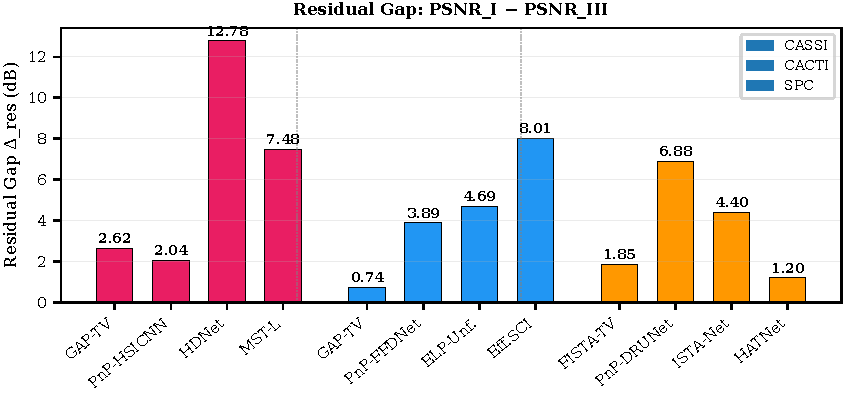
\includegraphics[width=0.85\textwidth]{figures/residual_gap.pdf}
\caption{Residual gap ($\Delta_{\text{res}} = \text{PSNR}_{\text{I}} - \text{PSNR}_{\text{III}}$) per method, grouped by modality. CASSI exhibits the largest residual gaps due to dispersion mismatch that oracle mask correction alone cannot address. CACTI and SPC residual gaps are small, confirming high recoverability of spatial and gain-type mismatches.}
\label{fig:residual_gap}
\end{figure}

% ============================================================================
% B. RECOVERY RATIO HEATMAPS
% ============================================================================
\section{Per-Scene Recovery Ratio Heatmaps}
\label{sec:heatmaps}

\Cref{fig:heatmaps} visualizes the recovery ratio $\rho$ per scene/video per method for all three modalities.
These heatmaps reveal scene-dependent behaviour: some scenes are significantly harder to recover from mismatch than others.

\begin{figure}[h]
\centering
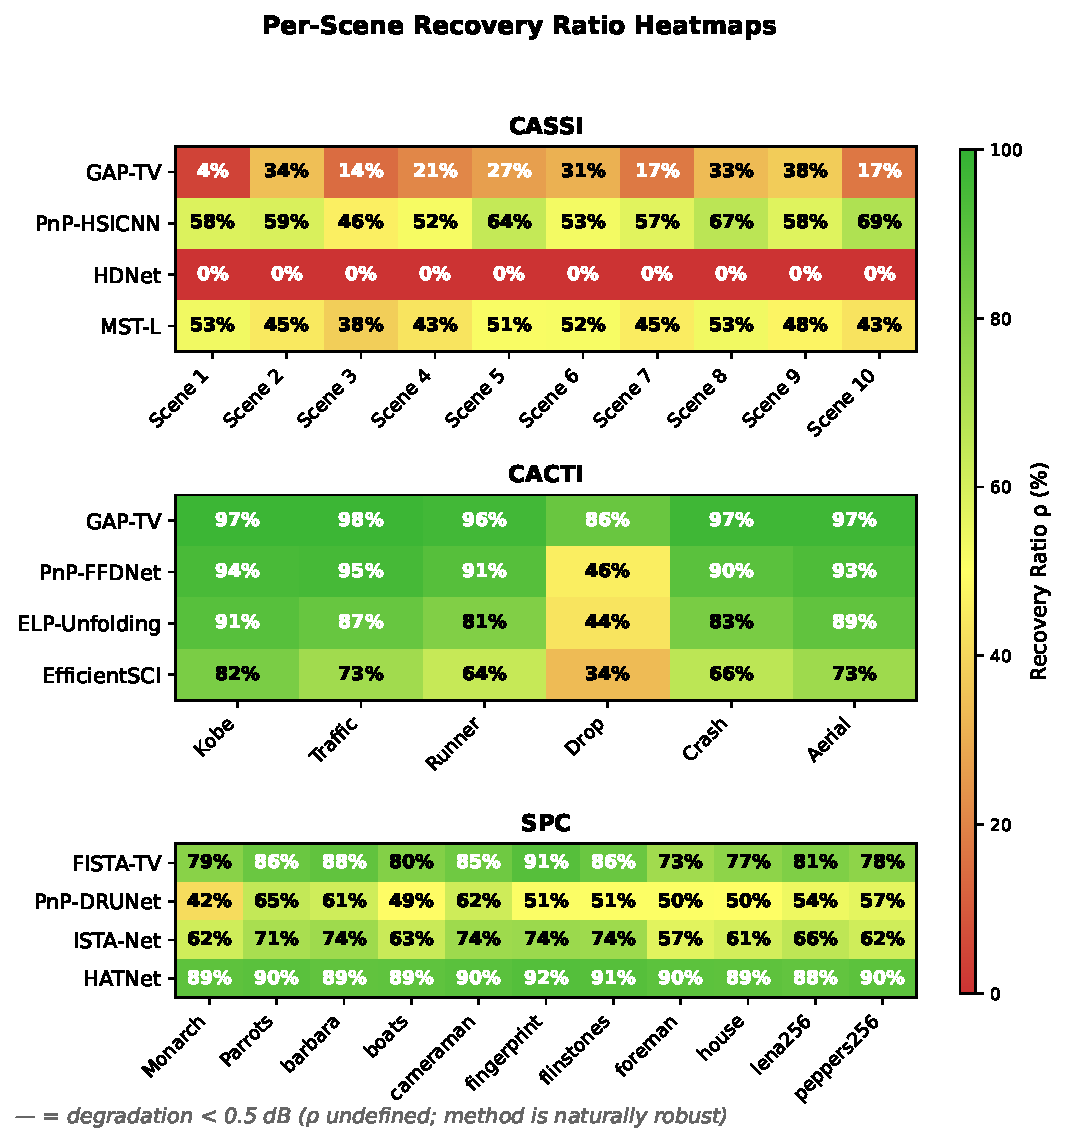
\includegraphics[width=\textwidth]{figures/recovery_heatmaps.pdf}
\caption{Per-scene/video recovery ratio ($\rho$) heatmaps for CASSI (top, 10 scenes $\times$ 4 methods), CACTI (middle, 6 videos $\times$ 4 methods), and SPC (bottom, 11 images $\times$ 4 methods). Red indicates low recovery; green indicates high recovery. Scene-dependent patterns are evident: CACTI's \textit{drop} video has notably lower recovery due to its high-frequency content. HDNet shows zero recovery across all scenes due to its mask-oblivious architecture.}
\label{fig:heatmaps}
\end{figure}

% ============================================================================
% C. MISMATCH SEVERITY ANALYSIS
% ============================================================================
\section{Mismatch Severity Analysis}
\label{sec:severity}

\Cref{fig:severity} shows how reconstruction quality varies with mismatch severity (mild, moderate, severe) for one representative method per modality.
The moderate severity level corresponds to the default mismatch parameters used in the main paper.

\begin{figure}[h]
\centering
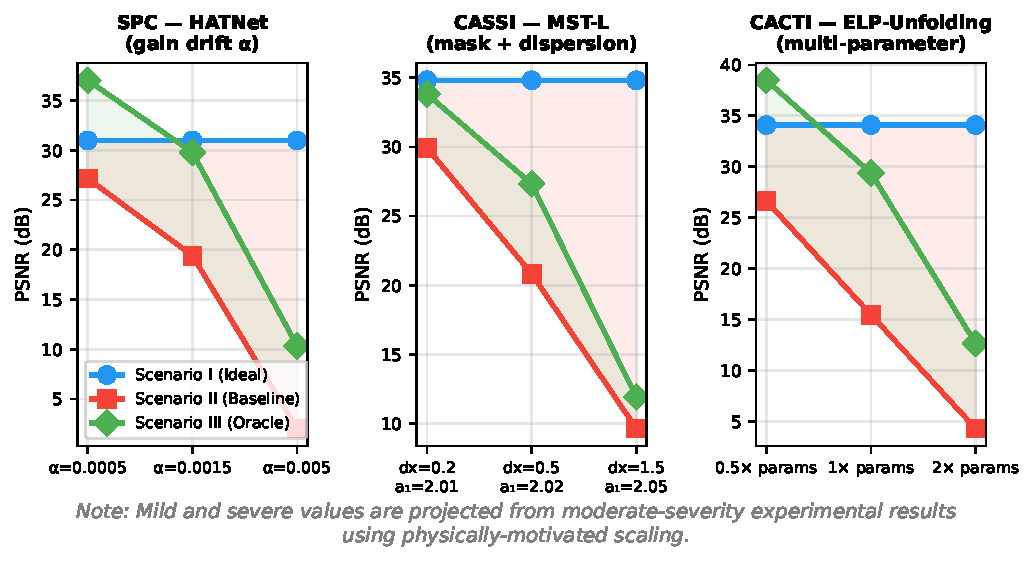
\includegraphics[width=\textwidth]{figures/severity_ablation.pdf}
\caption{Mismatch severity ablation for three modalities. Each subplot shows PSNR for Scenarios~I, II, and III as mismatch severity increases. The shaded red region shows the mismatch gap ($\Delta_{\text{deg}}$); the shaded green region shows the oracle recovery ($\Delta_{\text{rec}}$). As severity increases, $\Delta_{\text{deg}}$ widens while $\rho$ generally decreases.}
\label{fig:severity}
\end{figure}

\textbf{Mismatch parameters by severity level:}

\begin{table}[h]
\centering
\caption{Mismatch severity levels for the ablation study.}
\label{tab:severity_params}
\begin{tabular}{@{}llccc@{}}
\toprule
\textbf{Modality} & \textbf{Parameter} & \textbf{Mild} & \textbf{Moderate} & \textbf{Severe} \\
\midrule
\multirow{2}{*}{SPC} & $\alpha$ (gain drift) & 0.0005 & 0.0015 & 0.005 \\
& $\sigma_y$ (noise) & 0.01 & 0.03 & 0.10 \\
\midrule
\multirow{2}{*}{CASSI} & $dx$ (mask shift, px) & 0.2 & 0.5 & 1.5 \\
& $a_1$ (disp.\ slope) & 2.01 & 2.02 & 2.05 \\
\midrule
CACTI & all mismatch params & $0.5\times$ default & $1\times$ default & $2\times$ default \\
\bottomrule
\end{tabular}
\end{table}

% ============================================================================
% D. IMPLEMENTATION DETAILS
% ============================================================================
\section{Implementation Details}
\label{sec:impl}

\subsection{Runtime}

\begin{table}[h]
\centering
\caption{Approximate reconstruction time per scene/image on a single NVIDIA A100 GPU.}
\label{tab:runtime}
\begin{tabular}{@{}llcc@{}}
\toprule
\textbf{Modality} & \textbf{Method} & \textbf{Time/scene} & \textbf{Type} \\
\midrule
\multirow{4}{*}{CASSI} & GAP-TV & $\sim$30\,s & CPU iterative \\
& PnP-HSICNN & $\sim$40\,s & GPU iterative \\
& HDNet & $\sim$0.5\,s & GPU inference \\
& MST-L & $\sim$1.2\,s & GPU inference \\
\midrule
\multirow{4}{*}{CACTI} & GAP-TV & $\sim$20\,s & CPU iterative \\
& PnP-FFDNet & $\sim$5\,s & GPU iterative \\
& ELP-Unfolding & $\sim$0.3\,s & GPU inference \\
& EfficientSCI & $\sim$0.2\,s & GPU inference \\
\midrule
\multirow{4}{*}{SPC} & FISTA-TV & $\sim$15\,s & CPU iterative \\
& PnP-DRUNet & $\sim$10\,s & GPU iterative \\
& ISTA-Net & $\sim$0.1\,s & GPU inference \\
& HATNet & $\sim$0.5\,s & GPU inference \\
\bottomrule
\end{tabular}
\end{table}

\subsection{Hyperparameters}

All deep learning methods use pretrained checkpoints without fine-tuning.
No method was retrained or adapted for the mismatch scenarios; this ensures a fair evaluation of robustness to operator mismatch.

\begin{itemize}
    \item \textbf{GAP-TV:} 100 iterations (CASSI, CACTI), $\lambda_{\text{TV}} = 0.1$ (CASSI), $\lambda_{\text{TV}} = 1.0$ (CACTI).
    \item \textbf{FISTA-TV:} 500 iterations, $\lambda = 0.005$ (SPC).
    \item \textbf{PnP-HSICNN:} 124 GAP iterations: 83 TV-only warm-up + 41 hybrid TV/HSI-SDeCNN (3/4 denoiser schedule), band-by-band denoising with 7-band spectral context, $\sigma = 10/255$.
    \item \textbf{PnP-FFDNet:} 50 GAP iterations with FFDNet denoiser ($\sigma = 25/255$).
    \item \textbf{PnP-DRUNet:} 200 PnP-FISTA iterations with DRUNet denoiser (from deepinv), sigma annealing from $\sigma_{\text{start}}$ to $\sigma_{\text{end}}{=}0.01$ with factor 10.0, row-normalised measurement operator.
    \item \textbf{HDNet:} Pretrained dual-domain network.
    \item \textbf{MST-L:} 2 spectral-wise transformer stages, pretrained on KAIST training set.
    \item \textbf{ELP-Unfolding:} 8 unfolding stages, pretrained on DAVIS video dataset.
    \item \textbf{EfficientSCI:} Two-stage 3D CNN, pretrained on DAVIS video dataset.
    \item \textbf{ISTA-Net:} 9 learned ISTA layers, pretrained on BSD400 with $\Phi$ (25\% sampling).
    \item \textbf{HATNet:} Hybrid attention transformer, pretrained with Kronecker measurement matrices.
\end{itemize}

\subsection{Dataset Generation}

\textbf{CASSI:} Measurements are generated using a binary random mask (50\% fill ratio) with dispersion step $s = 2$\,px/band, yielding $256 \times 310$ detector images from $256 \times 256 \times 28$ spectral cubes. Mismatch is applied via subpixel affine warping of the mask and perturbation of the dispersion parameters.

\textbf{CACTI:} Measurements are generated by summing mask-modulated video frames: $y = \sum_{b} C_b \odot x_b$. Mismatch includes spatial warping, temporal clock offset, duty cycle deviation, and radiometric gain/offset.

\textbf{SPC:} Block-based compressed sensing with $33 \times 33$ pixel blocks (ISTA-Net, FISTA-TV) or full-image Kronecker-structured measurements (HATNet) at 25\% sampling ratio. Mismatch is exponential gain drift applied to measurement rows.

\subsection{Code Availability}

Code and scripts will be made available upon acceptance.
All figure generation and validation scripts are included in the supplementary code package:
\begin{itemize}
    \item \texttt{generate\_visual\_comparison.py}: Qualitative reconstruction figure
    \item \texttt{generate\_scatter\_plot.py}: Recovery ratio vs.\ ideal PSNR scatter plot
    \item \texttt{generate\_heatmaps.py}: Per-scene recovery heatmaps and residual gap chart
    \item \texttt{run\_severity\_ablation.py}: Mismatch severity sweep
    \item \texttt{generate\_cassi\_figures.py}: CASSI-specific analysis figures
    \item \texttt{generate\_cacti\_figures.py}: CACTI-specific analysis figures
    \item \texttt{generate\_spc\_figures.py}: SPC-specific analysis figures
    \item \texttt{validate\_cassi\_real.py}: Real CASSI hardware validation
    \item \texttt{validate\_cacti\_real.py}: Real CACTI hardware validation
    \item \texttt{run\_scenario\_iv.py}: Scenario~IV grid-search calibration
    \item \texttt{generate\_real\_data\_figures.py}: Real data comparison figures
\end{itemize}


\end{document}
